%%%%%%%%%%%%%%
% Fichero: uclmTFGesi.tex
% Autor: Jesús Salido Tercero (http://www.uclm.es/profesorado/jsalido)
% Fecha (creación): Febrero 2010 
% Rev. : Febrero 2019
% Descripción: Plantilla para memoria de TFG 
% (Escuela Sup. de Informática, UCLM). Creada para el curso 
% “LaTeX esencial para preparación de TFG, Tesis y otros documentos 
% académicos” (Esc. Sup. Informática-UCLM)
%
%### Compilación 
%
%Esta plantilla ha sido preparada para compilarse con `pdflatex`, `biblatex` 
%(bibliografía con `biber`) y `makeindex` (sólo si se incluye índice 
%temático).
%
%Para su compilación se aconseja utilizar `latexmk` (requiere para su 
%ejecución de un intérprete [`Perl`](http://strawberryperl.com/)):
%
%> \$> latexmk -pdf -silent -synctex=1 --enable-write18 
%
%Para la automatización del trabajo con esta plantilla es recomendable el 
%empleo de IDE dedicados como [TeXstudio](https://www.texstudio.org/).
%
% Una versión actualizada de esta plantilla está disponible en overleaf.
% Puede crearse un proyecto propio para escribir un TFG directamente en overleaf,
% o bien descargarla como un archivo .zip para su utilización en modo local.
%
% Si deseas acceder a la versión de desarrollo puedes encontrarla en GitHub:
%	https://github.com/JesusSalido/TFG_ESI_UCLM
%%%%%%%%%%%%%%


% -------------------------
%
% PREÁMBULO del documento
%
% -------------------------
	
\documentclass[ 		% Clase del documento
	11pt,				% Tamaño de letra
	a4paper,			% Tamaño de papel
	twoside,			% Impresión a doble cara
	openright,			% La apertura de cap. a la dcha.
	final       		% Versión final
]{book}

\usepackage[utf8]{inputenx} % Codificación de entrada
\usepackage[english,spanish,es-tabla,es-noindentfirst]{babel} % Internacionalización

%--- Geometría de las páginas del documento
\usepackage[			% Márgenes del documento
	top=2.5cm,			% Margen superior
	bottom=2.5cm,		% Margen inferior
	inner=3.5cm,		% Margen al interior
	outer=2cm			% Margen al exterior
]{geometry}


%--- Tipografía
\usepackage{textcomp,marvosym,pifont} % OPT.: Generación de símbolos 
%especiales
\usepackage{ccicons} % OPT.: Iconos de licencia Creative Commons
\usepackage{amsmath,amsthm,amssymb}	% OPT.: Mejoras cuando hay matemáticas



%--- Tipografía (Opción 1)
\usepackage[tt=false]{libertine}	% Libertine
\usepackage[libertine]{newtxmath}	% Times
%---


%--- Tipografía (Opción 2)
%\usepackage{newpxtext}				% Palatino: La opción osf proporciona números en old style.
%\usepackage{newpxmath}				% Palatino
%---


\usepackage[T1]{fontenc}% Codificación de salida    
\usepackage{microtype}	% Mejoras de microtipografía en la obtención de PDF (sólo para pdflatex)


%--- Paquete con personalización local para el TFG (ESI-UCLM)
% EDITAR: Si es preciso que la memoria emplee "english" como idioma 
% principal y prefijos de género.
% Con la opción "english" el resto de opciones son irrelevantes.
% Ejemplos: 
% 	\usepackage{uclmTFGesi} % Memoria en español y prefijos masculinos.
\usepackage[autora]{uclmTFGesi} % Memoria en español y autora.
%  	\usepackage[english]{uclmTFGesi} % Memoria en inglés.
%\usepackage{uclmTFGesi} % Opción de idioma de la memoria y prefijos de género.


%--- Gráficos y tablas
\usepackage{graphicx}	% Inclusión de figuras
\usepackage{booktabs}   % Para las tablas
\usepackage{subfigure}	% OPT.: Inclusión de subfiguras
% EDITAR: Si es necesario cambiar el path para los directorios de figuras.
\graphicspath{{./figs/}}% Path de búsqueda de ficheros gráficos
\DeclareGraphicsExtensions{.pdf,.png,.jpg} % Precedencia de extensiones
\usepackage{rotating}	% OPT.: Giro de cajas (texto, figuras, tablas) (No 
%DVI)
\usepackage{tabularx,booktabs}	% OPT.: Ajustes para tablas


%--- Personalización de títulos de figuras y tablas
\usepackage[%
	margin=10pt,		% Margen
	font=small,			% Tamaño de tipografía
	labelfont=bf,		% Prefijo-Etiqueta en negrita
	format=hang			%
]{caption}
\captionsetup[table]{skip=4pt} 	% Separación del caption en las tablas


%--- Bibliografía: Biblatex con biber.
\usepackage[
	backend=biber, 		% Backend
	sortcites,
	defernumbers=true, 	% Para numerar al final
	style=numeric-comp, % Estilo numérico condensado
	% Descomentar las opciones siguientes para bibliografía multilingüe
%	autolang=other, 	% Requerido para opción multilingüe
%	language=auto   	% Requerido para opción multilingüe
]{biblatex}

% Línea añadida para eliminar el idioma de la fuente bibliográfica.
\AtEveryBibitem{\clearfield{note} \clearlist{language}}
% OJO: Editar si se cambia el fichero de bibliografía. 
\addbibresource{biblioTFG.bib} 	% Fichero de bibliografía.
%---

\usepackage{makeidx} % OPT.: Indice temático
\makeindex           % OPT.: Procesamiento de índice temático


%--- OPT.: Paquete para incluir menús, paths y teclas de modo "elegante"
\usepackage[os=win,hyperrefcolorlinks]{menukeys} 
\usepackage{todonotes}
%--- Paquete para poder añadir acrónimos
\usepackage[acronym]{glossaries}
\makeglossaries

\newacronym{api}{API}{Application Programming Interface}
\newacronym{eso}{ESO}{Educación Secundaria Obligatoria}
\newacronym{pud}{PUD}{Proceso Unificado de Desarrollo}
\newacronym{ide}{IDE}{Integrated Development Environment} % Índice de acrónimos usados
% OJO: Este paquete presenta algunas incompatibilidades, debe cargarse el 
%último y exige la desactivación de la opción colorlinks y la inclusión en 
%este paquete de la opción hyperrefcolorlinks.
% Este paquete presenta alguna incompatibilidades por lo que cambiarlo de 
%ubicación puede generar algún error (manejar con cuidado).

% Estas definiciones permiten cambiar el estilo de los elementos. Si se desean otros estilos o su configuación es preciso recurrir a la documentación del paquete (no lo recomiendo).
\renewmenumacro{\menu}[>]{menus} % OPT.: default: menus
\renewmenumacro{\directory}[/]{pathswithblackfolder} % OPT.: default: paths
\renewmenumacro{\keys}[+]{shadowedroundedkeys} % OPT.: default: roundedkeys
%---

% -------------------------
% -------------------------
% -------------------------



% -------------------------
% -------------------------
% -------------------------
% DATOS DEL DOCUMENTO 
% Definición de variables empleadas en el documento por lo que no son
% traducidos. Cuando algún campo puede tener varias líneas aparecen dos
% campos señalados como <campo>Primera y <campo>Segunda. Si no se desea 
% emplear los campos opcionales (OPT.) estos deben comentarse.
% -------------------------
% EDITAR: Datos del documento. 
% NOTA: Los elementos opcionales pueden eliminarse o comentarse.
\tituloPrimera{TeachHelper} % 1ª Línea
\tituloSegunda{Aplicación para los maestros} % OPT.: Para títulos largos.
%%existe).
\titulo{TeachHelper} % Título corto (no mostrado en portada)
\autor{Lucía Calzado Piedrabuena}
\email{lucia.calzado1@alu.uclm.es}					
\tutor{María del Carmen Lacave Rodero}
%\cotutor{<co-tutor(a) (nombre apellidos)>}	% OPT.: Cotutor(a)
\instEdu{UNIVERSIDAD DE CASTILLA-LA MANCHA}

% Fichero con escudo de la institución
% Logo de la ESI que prefieras (la normativa no especifica obligatoriedad).
%\escudo{esi} 			% Logo ESI (gris uniforme)							
%\escudo{esi_black} 	% Logo ESI (negro)						
%\escudo{esi_color}		% Logo ESI (dos tintas)						
\escudo{escudoInf}		% Nucleo de ferrita	(color)
%\escudo{escudoInfBW} 	% Nucleo de ferrita	(en escala de grises)					
%\escudo{etsii} 		% Ejemplo para otra titulación

\centroEdu{ESCUELA SUPERIOR DE INFORMÁTICA}
\deptoEduPrimera{<Primera línea Depto. Director>} % 1ª Línea
\deptoEduSegunda{<Segunda línea Depto. Director>} % OPT.: Para nombres largos.
\titulacion{GRADO EN INGENIERÍA INFORMÁTICA}
\especialidad{Computación} % OPT.: Especialidad - Intensificación
\tipoDoc{TRABAJO FIN DE GRADO}

% Si las fechas se desean en inglés hay que ponerla explícita.
\fechaDef{insertarMes, 2020} 					% Fecha de defensa
\mesDef{insertarMes}        					% Mes de defensa
\yearDef{2020}        							% Año de defensa
\lugarDef{Ciudad Real}							% Lugar de defensa


% --- Metadatos (propiedades) para el documento PDF
\hypersetup{% OPT.
% EDITAR: Valores para el PDF.	
	pdftitle={Título}, % Título
	pdfauthor={Autor}, % Autor
	pdfsubject={TFG},  % Tema
	pdftoolbar=true, % Muestra la toolbar de Acrobat
	pdfmenubar=true	 % Muestra la menubar de Acrobat
}
% -------------------------
% -------------------------
% -------------------------



% -------------------------
%
% CUERPO DEL DOCUMENTO
%
% -------------------------
\begin{document}
\frontmatter
% Cambia la numeración de páginas a números romanos y las secciones no están 
%numeradas aunque si aparecen en el índice de contenidos.
\pagestyle{empty}  % Páginas sin cabecera ni pies

% -------------------------
%
% PORTADAS
%
% -------------------------
\portadaTFG		% Portada pral.
%---
\portadillaTFG	% Portada interior (con tutor(a) y co-tutor(a) si existe).
%---

% -------------------------
%
% CRÉDITOS
%
% -------------------------
% -------------------------
%
% CRÉDITOS
%
% -------------------------
% EDITAR (opcional): Licencia (si se desea modificar).
% Este comando permite una gran flexibilidad y la ventaja de no depender de paquetes externos.
% Esta es una página reservada para señalar información relativa a los derechos de autor y la licencia de distribución y uso del documento. Esta página debería ser aprovechada también para informar de cualquier tipo de cesión de los derechos anteriormente citados. El autor del TFG debe tener presente que el incumplimiento de la legislación vigente en materia de protección de la propiedad intelectual es de su exclusiva responsabilidad independientemente de la cesión de derechos que este haya convenido para su obra ya que no son objeto de cesión aquellos derechos de los que no se es poseedor.

\creditos{Este documento se distribuye con licencia Creative Commons Atribución Compartir Igual 4.0. El texto completo de la licencia puede obtenerse en \url{https://creativecommons.org/licenses/by-sa/4.0/}. 
% El escudo de Informática basado en el núcleo de ferrita que acompaña la distribución de esta plantilla ha sido realizado por P.~Moya, D.~Villa e I. Díez, su inclusión debe respetar los derechos de autor y las licencias a las que se vea sometido. 

La copia y distribución de esta obra está permitida en todo el mundo, sin regalías y por cualquier medio, siempre que esta nota sea preservada. Se concede permiso para copiar y distribuir traducciones de este libro desde el español original a otro idioma, siempre que la traducción sea aprobada por el autor del libro y tanto el aviso de copyright como esta nota de permiso, sean preservados en todas las copias.}{cclicense}
%---



%---
\tribunalTFG % Página para calificaciones del tribunal
%---

% -------------------------
%
% OPT.: DEDICATORIA (1 pág. máximo) comentar si no se desea incluir.
% Aunque opcional, no se debería perder la oportunidad de poder 
% dedicar el trabajo a alguien MUY especial.
% EDITAR: Dedicatoria.
\dedicado{A mi madre, \\ % A alguien muy especial
por el inmenso amor a su trabajo.} % Como mucho dos líneas (no confundir con los agradecimientos).
% -------------------------

% -------------------------
%
% RESUMEN:
%
% -------------------------
\listoftodos
%--- Ajustes del documento.
\pagestyle{plain}	% Páginas sólo con numeración inferior al pie

% -------------------------
%
% RESUMEN:
% OJO: Si es preciso cambiar manualmente orden Resumen <-> Abstract
%
% -------------------------
%--- Resumen en español
\selectlanguage{spanish} % Selección de idioma del resumen.
\cleardoublepage % Se incluye para modificar el contador de página antes de añadir bookmark
\phantomsection  % OJO: Necesario con hyperref
\pdfbookmark[0]{Resumen}{idx_resumen}% idx_resumen.0 % Bookmark en PDF

\begin{abstract}
% EDITAR: Resumen (máx. 1 pág.)
\begin{center}
\emph{TeachHelper}
\end{center}
Este Trabajo de Fin de Grado consiste en el desarrollo de una aplicación para escritorio que apuesta por la comodidad y conveniencia de los maestros a la hora de almacenar las calificaciones de sus alumnos.
\newline
Dicha aplicación, desarrollada en Java mediante una metodología en cascada, consistirá en un asistente que el maestro ejecutará para guardar las pruebas, notas, competencias y observaciones de sus alumnos, ordenados por asignaturas y cursos.
\newline

\end{abstract}
%---

%--- Ajuste del idioma para el resto del documento.
\ifspanish
	\selectlanguage{spanish}% Emplea idioma español
\else
	\selectlanguage{english}% Emplea idioma inglés
\fi

%---

% -------------------------
%
% AGRADECIMIENTOS (recomendable máx. 1 pág.)
%
% -------------------------
\ifspanish
	\selectlanguage{spanish}
\else
	\selectlanguage{english}
\fi

% -------------------------
%
% AGRADECIMIENTOS (recomendable máx. 1 pág.)
%
% -------------------------
\cleardoublepage
\phantomsection % OJO: Necesario con hyperref
\pdfbookmark[0]{Agradecimientos}{idx_agrad}% idx_agrad.0 % Bookmark en PDF

\chapter*{Agradecimientos} % Opción con * para que no aparezca en TOC ni numerada

Escribir algo aquí si eso

\makeatletter		
\begin{flushright}
	\textit{\@autor}
\end{flushright}
\makeatother % Agradecimientos etc.
%---

%--- MAINMATTER
% Capítulos del documento
% Salva en un contador interno el nº de páginas actual
% Debe ir antes de \mainmatter (antes de que se reinicie el cnt page)
\savepagecnt
\mainmatter
% Justo antes del primer capítulo del libro. Activa la numeración con números arábigos y reinicia el contador de páginas.

% OJO: No cambiar de ubicación. Elimina cabecera y pie en pág. inicial de cap.
\cleanhdfirst

% Reajuste del número de página consecutivo para no reiniciar paginación en Cáp. 1
%\contpagination % Comentado para reiniciar paginación (pag. 1)

% -------------------------
%
% CAPÍTULOS: Un fichero por capítulo.
%
% -------------------------
\chapter{Introducción}
\label{cap:Introduccion}

Este trabajo va dirigido a los maestros de Educación Secundaria Obligatoria (ESO), consistente en la creación de una herramienta software donde puedan almacenar los datos de sus alumnos así como sus calificaciones a lo largo del curso.

A día de hoy, la mayoría de los maestros siguen usando hojas de cálculo para almacenar las calificaciones de sus alumnos. Esto, aunque es una mejor opción que hacerlo a mano, todavía dista mucho de ser una herramienta fácil de usar para cualquier persona, transparente para el maestro y visualmente agradable.

Para ello, se quiere crear una aplicación que, si bien permitirá a los profesionales docentes hacer el seguimiento de las calificaciones de sus alumnos, lo hará de forma simple e intuitiva, reduciendo el tiempo requerido para la tarea y haciéndola más amena.

\section{Usuarios}

Los usuarios de la aplicación serán los maestros de Educación Secundaria Obligatoria.

\section{Aplicaciones existentes}

En este apartado se describen aplicaciones existentes y actuales que hacen lo mismo que la mía pero la mía es mejor por las razones que voy a exponer a continuación.

\subsection{EducamosCLM (Papás 2.0)}

Esta aplicación web de la Junta de Comunidades de Castilla-La Mancha es la aplicación de gestión de alumnado por excelencia en los colegios públicos. 

Características:

\begin{enumerate}
    \item \textbf{Planificación semanal.}
    Un calendario y una agenda personales que tanto los alumnos como los profesores pueden usar para planificar los estudios, los exámenes o controles, trabajos o cualquier otro hito de la semana. También cuenta con un sistema de citaciones y reuniones.
    \item \textbf{Seguimiento del curso.}
    En este apartado, los profesores pueden publicar las notas de sus alumnos para que estos y sus padres las vean en cualquier momento, así como las faltas de asistencia y la trayectoria escolar que lleva el alumno durante el curso.
    En la vista de los alumnos, estos podrán subir sus trabajos online, que le aparecerán al profesor para que pueda descargarlos, calificarlos e introducir dicha calificación en el sistema, así como pedir tutorías con los profesores.
    \item \textbf{Comunicaciones con los padres y alumnos.}
    Un sistema de mensajería para que los profesores puedan mantenerse en contacto con los padres y los alumnos.
    \item \textbf{Características menores.}
        \begin{itemize}
            \item Documentos solicitados: los profesores pueden solicitar mediante esta característica documentos a los padres (justificantes de asistencia, exámenes firmados...)
            \item Tablón de anuncios: aquí los profesores pueden escribir avisos que van en forma de notificaciones a los alumnos y los padres.
            \item Secretaría virtual: esta aplicación también cuenta con un enlace a la secretaría virtual. Desde aquí se controlan los alumnos nuevos, entre muchas otras gestiones, a nivel de Centro.
        \end{itemize}
\end{enumerate}
        
En qué podría mejorar mi aplicación respecto a esta:

\begin{enumerate}
    \item \textbf{No depende del Centro}. TeachHelper es una aplicación libre, que no está unida a la Junta de Comunidades. Es una aplicación individual con varios niveles de personalización.
    \item \textbf{Más simple}. Mientras que EducamosCLM tiene características especiales que permiten la comunicación con los padres y un alto nivel de personalización de tareas, TeachHelper es mucho más sencillo, intuitivo y fácil de usar, a la vez que mantiene una alta personalización.
    \item \textbf{Personalizado para cada maestro/a}. TeachHelper tiene una característica única: guarda y aprende de las preferencias y los cursos más usados por cada maestro/a, para sugerirlas la próxima vez que entre a la aplicación.
\end{enumerate}

\subsection{Google Classroom}

Aplicación de navegador y de smartphone desarrollada por Google que permite la comunicación entre profesores y alumnos, así como la gestión y organización de trabajos mediante Google Drive.

Características:

\begin{enumerate}
	\item \textbf{Fácil e intuitivo}. Pensado tanto para profesores como para alumnos, Google Classroom es fácil de usar. Tiene herramientas para programar entregas, reuniones y hablar con todo el grupo de alumnos a la vez mediante texto. Además, permite subir archivos a la nube para ser calificados por los profesores.
	\item \textbf{Todo en la nube}. Todos los archivos que se suben van directamente a Google Drive. De esta forma, se tienen todos juntos, pero ordenados.
	\item \textbf{Integración con otras aplicaciones}. Google Classroom permite la integración de aplicaciones como Classcraft, Pear Deck o Quizizz, permitiendo una completa personalización de la experiencia tanto para los alumnos como para los maestros. Esto le da flexibilidad a la aplicación.
	\item \textbf{Accesible para primaria, secundaria o educación superior}. Debido a la generalización de la herramienta, es muy versátil y se puede usar para cualquier curso.
\end{enumerate}

En qué podría mejorar mi aplicación respecto a esta:

\begin{enumerate}
	\item \textbf{Más orientada a los profesores}. Google Classroom es una herramienta orientada a ayudar a dar clase a los profesores. Tiene varias funcionalidades que permiten, por ejemplo, que varios alumnos trabajen en el mismo documento. Esto sale un poco del propósito de TeachHelper, que es el de organización de los documentos del profesorado, no de las propias clases.
	\item \textbf{Cuenta de Google}. Para usar Google Classroom, tanto el alumno como el profesor necesitan tener una cuenta de Google, y eso es algo que no recomiendan todos los Centros, sobre todo si son públicos, por motivos de seguridad de los datos. Cada usuario de Google Classroom debería hacerse una cuenta específica para usarlo. TeachHelper solo va dedicada a los maestros, y solo ellos deberán registrarse.
	\item \textbf{Personalización}. De nuevo, TeachHelper cuenta con la característica de la personalización dependiendo del maestro/a que Classroom no tiene, por el enfoque de la aplicación.
\end{enumerate}
	

\subsection{Additio}

Aplicación de navegador y de smartphone que permite gestionar las notas del alumnado y las competencias que tiene cada metodología, planificar las clases y la comunicación con padres y alumnos.

Características:

\begin{enumerate}
	\item \textbf{Una aplicación potente}. Additio es, de las aplicaciones de las que hemos hablado hasta ahora, la que más se parece a la idea de TeachHelper. Diseñada para profesores como para Centros, permite gestionar notas y trabajos, la asistencia a clase y la comunicación entre padres, profesores y alumnos. 
	\item \textbf{Apartado de cálculo de competencias}. Una de las características de esta aplicación es que permite establecer las competencias de una prueba, a las que se les puede dar peso para calcular notas.
	\item \textbf{Calendario y agenda}. Additio tiene un calendario y una agenda para establecer citas con alumnos o padres.
	\item \textbf{Para Centros y para profesores}. Se pueden contratar dos tipos de aplicaciones: una para el Centro y otra para el profesor.
	\item \textbf{Informes}. Permite sacar informes de cualquier alumno para ver la trayectoria a lo largo de los trimestres.
\end{enumerate}

En qué podría mejorar mi aplicación respecto a esta:

\begin{enumerate}
	\item \textbf{Demasiadas características}. Aunque es una aplicación, como hemos mencionado anteriormente, muy potente, quizá ese sea su punto débil: es muy extensa. TeachHelper está enfocada a ayudar con la gestión de las notas del alumnado y es mucho más simple de utilizar.
	\item \textbf{Pensada principalmente para tablet y smartphone}. En su página web mencionan que esta aplicación está pensada para los profesores que usen su tablet o smartphone como forma principal de gestionar sus clases. TeachHelper es una aplicación de escritorio porque a todos los maestros se les da un ordenador portátil en el trabajo.

\end{enumerate}
\chapter{Objetivo}
\label{cap:Objetivo}

Los maestros de \gls{eso}... 
\todo{chapter Objetivo}
<<Escribir aquí cosas como que pues que necesitan algo para tener sus notas todas en un sitio y que sea más ''conveniente'' que una hoja de Excel>>

Problema que se plantea: los maestros de \gls{eso} necesitan alguna forma de guardar las calificaciones de los alumnos de forma ergonómica y sencilla.

Es interesante solucionar este problema porque: 
\todo{chapter Objetivo}
<<Escribir aquí cosas como que los profesores aunque tienen el Papás, podrían usar otro tipo de herramienta que no dependiera de si son afiliados al Gobierno o no... Algo así?>>

\section{Funcionalidades de la aplicación} \label{funcionalidades}

La aplicación podrá permitir a los maestros:
\begin{enumerate}
	\item \textbf{Iniciar sesión} mediante un usuario y una contraseña únicos para cada maestro.
	\item \textbf{Gestionar y calificar las distintas tareas y pruebas de los alumnos}. Mediante una tabla en la ventana principal, los maestros podrán calificar los exámenes, pruebas y tareas de sus alumnos. La aplicación calculará las notas finales dependiendo de la ponderación que se le dé a las tareas. También se gestionarán las competencias que tiene cada asignatura y cada prueba.
	\item \textbf{Gestionar sus alumnos}. Cada alumno pertenece a un curso y a varias asignaturas. Todo esto se gestionará gracias a la base de datos.
	\item \textbf{Gestionar las competencias de las asignaturas}. Cada asignatura tendrá unas competencias con sus ponderaciones. Una prueba tendrá unas competencias determinadas, relacionadas con la asignatura. Esto también se gestiona desde la base de datos.
	\item \textbf{Añadir comentarios a los alumnos} sobre su asistencia, comportamiento, o cualquier punto que el maestro considere oportuno.
	\item \textbf{Obtener recomendaciones de forma dinámica} sobre las asignaturas en las que se debería trabajar (o que, por ejemplo, aún no se han introducido datos), alumnos que mejoran o empeoran a lo largo del curso o tablas que se han dejado a medias.
	\item \textbf{Visualizar informes del alumno} para ver su trayectoria escolar durante todo el año.
	

\end{enumerate}


%\include{AnalisisAppsExistentes}
\chapter{Metodología y método de trabajo}
\label{cap:metodologia}

En este capítulo se explica la metodología de desarrollo que se ha seguido, describiendo desde la captura de requisitos hasta el producto final. Al final del capítulo se añade un apartado con el análisis de costes.

\section{Metodología de desarrollo}

Para organizar el proyecto y permitir un desarrollo eficaz e incremental se ha seguido una metodología de desarrollo en espiral: el \gls{pud}\cite{pud} y \cite{apuntes}.

\subsection{Características principales}
El \gls{pud} es una metodología de desarrollo que transforma los requisitos de usuario en un sistema software. Es muy genérica, y por eso se ha decidido adaptar a este proyecto.
Las características básicas del \gls{pud} son las siguientes:
\begin{itemize}
	\item \textbf{Dirigido por casos de uso:} en este proyecto, los usuarios, como se ha mencionado anteriormente, son los maestros y profesores de \gls{eso}. Los casos de uso que se han contemplado para el proyecto son las acciones que se han especificado en \ref{cap:Introduccion}. Se hablará de la metodología seguida para la captura de requisitos más adelante.
	\item \textbf{Centrado en la arquitectura:} una de las primeras fases del proyecto es realizar el esquema de la base de datos y la comprensión de la futura arquitectura del programa. Esto determinará el orden en el que se desarrollarán los casos de uso.
	\item \textbf{Iterativo e incremental:} se ha trabajado mediante iteraciones, en la que cada una o bien añadía una nueva funcionalidad, mejoraba una de las ya existentes, o realizaba pruebas de cohesión entre los módulos recién añadidos y los que ya estaban desarrollados. También cabe notar que el método de iteraciones ha sido el de terminar por completo una parte, hasta las pruebas, antes de comenzar con otra nueva. En cada iteración en la que se añade una nueva funcionalidad:
	\begin{enumerate}
		\item Se elige una de las que todavía no se han desarrollado.
		\item Dentro de la funcionalidad, se identifican y especifican los casos de uso que le corresponden.
		\item Se refinan los diseños que se hicieron al principio del proyecto para estos casos de uso.
		\item Se implementan y se prueban dentro del módulo de manera que satisfaga de manera vaga los requisitos.
	\end{enumerate}
	
	En cada iteración en la que se mejora una funcionalidad existente:
	\begin{enumerate}
		\item Se elige una de las funcionalidades a probar.
		\item Se prueba exhaustivamente dentro de su módulo para identificar los errores actuales y posibles futuros, y se arreglan los fallos.
	\end{enumerate}
	
	En cada iteración en la que se prueba la cohesión entre los módulos:
	\begin{enumerate}
		\item Se elige uno de los módulos, preferentemente el último que se ha desarrollado.
		\item Se prueba con el resto de los módulos con los que mantiene cualquier tipo de comunicación, se identifican los errores y se arreglan los fallos.
	\end{enumerate}
	
	\item \textbf{Enfocado en los riesgos:} primero se han desarrollado los casos de uso más grandes que, después del primer diseño, se consideró que tendrían más impacto en el programa. Seguidamente, se fue trabajando desarrollando los distintos módulos, uno por cada funcionalidad y una iteración por funcionalidad.
	
\end{itemize}

\subsection{Etapas del proyecto}

Esta metodología consiste en la división del proyecto en cuatro etapas:
\begin{itemize}
    \item \textbf{Inicio:} para comenzar, se han recogido todos los requisitos y se ha estimado el alcance del proyecto. En esta etapa también se hizo la investigación de las aplicaciones ya existentes, descritas en el capítulo \ref{cap:aplicacionesexistentes} y el análisis de costes, desglosado en la sección \ref{analisiscostes}.
    \item \textbf{Elaboración:} se hicieron prototipos de las interfaces, se diseñó el software mediante diagramas y se estimaron las iteraciones a seguir.
    \item \textbf{Construcción:} se escribió el software según el resultado de la fase de elaboración, siguiendo las iteraciones previamente calculadas. 
    \item \textbf{Transición:} para finalizar se probó el producto final y se dio fin al desarrollo.
\end{itemize}

\subsection{Obtención de requisitos}
\label{sub:obtencionrequisitos}

Para la obtención y clasificación de los requisitos, se optará por varias metodologías:
\begin{itemize}
	\item \textbf{Observación activa:} se estudiará el entorno de trabajo del usuario final. Para ello, se realizó una sesión en la que se monitorizó a un usuario usando una de las herramientas descritas en el capítulo Aplicaciones existentes, preguntándole sus opiniones sobre algunas de las características que estaba utilizando.
	\item \textbf{Entrevistas:} entrevistas con el usuario en las que irá evaluando el producto final de cada sprint y añadiendo o modificando características.
\end{itemize}

Además, se ha aplicado la regla MoSCoW para priorizar el desarrollo de los requisitos funcionales. Esta regla divide los requisitos en cuatro categorías:
\begin{enumerate}
	\item \textbf{Must have (M):} requisitos que la aplicación debe tener y son prioritarios a cualquier otro de menor rango.	
	\item \textbf{Should have (S):} estos requisitos, de menor rango que los Must have, siguen siendo requisitos importantes para el desarrollo de la aplicación.	
	\item \textbf{Could have (C):} requisitos de más baja prioridad, que pueden posponerse si hay otros de mayor rango por encima de ellos.	
	\item \textbf{Won't have (W):} requisitos completamente opcionales que la aplicación podría llegar a tener de manera que mejorasen las funcionalidades.
	
\end{enumerate}

\section{Sprints}

A continuación se detallan los sprints que se realizaron en el proyecto. Cabe notar que este documento se escribió al mismo tiempo que se iban desarrollando.

El proyecto, que ha tenido una duración aproximada de 350 horas, se ha desarrollado desde el 2 de octubre de 2020 hasta el 1 de julio de 2021.

\subsection{Primer sprint - 2oct/1nov}

En el primer sprint (2 octubre 2020 - 1 noviembre 2020), al que se dedicaron 30 horas, se refinaron los diseños de la aplicación con la herramienta Balsamiq Wireframes [Sección \ref{sec:prototipos}]. Estos diseños se han modificado varias veces a lo largo de este primer sprint. Además, se realizó el primer diseño de la base de datos [Figura \ref{Fig:db_definition1}].

\begin{figure}[h]
\centering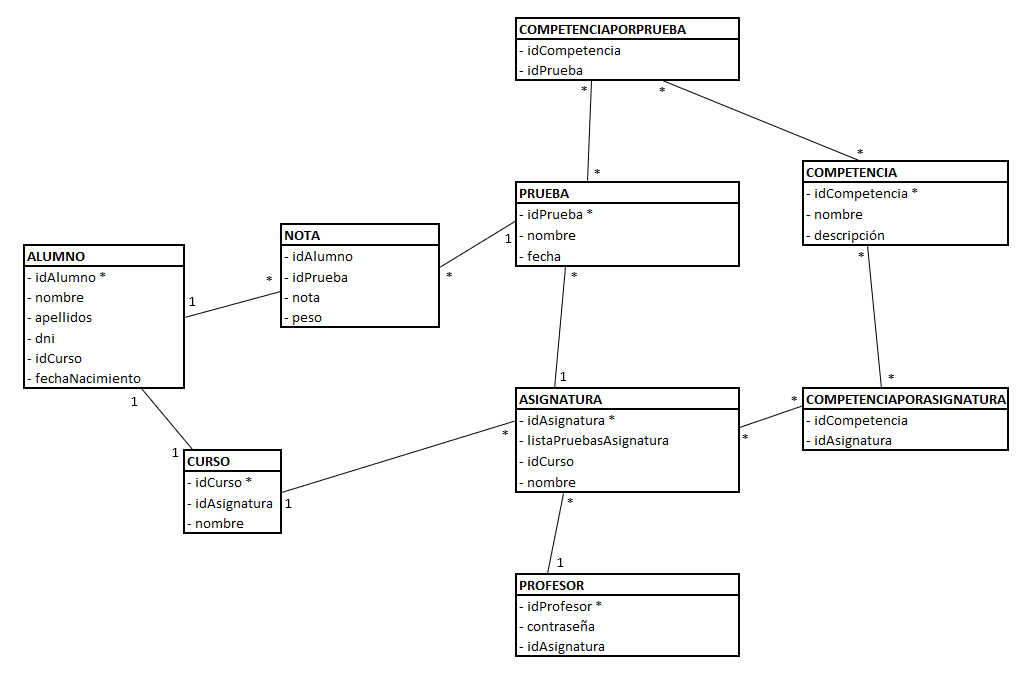
\includegraphics[width=1\linewidth]{figs/DB_Definition_1.png}
\caption{Primera definición de la base de datos.}
\label{Fig:db_definition1}
\end{figure}

\subsection{Segundo sprint - 2nov/1dic}

En el segundo sprint (2 noviembre 2020 - 1 diciembre 2020), al que se dedicaron 20 horas, se comenzó a escribir la memoria del proyecto, empezando por describir las aplicaciones existentes investigadas.

Se siguió trabajando en la base de datos, implementándola mediante MySQL [Sección \ref{sub:mysql}], y comenzó a poblarse de datos de prueba para comenzar el desarrollo.


\subsection{Tercer sprint - 2dic/1ene}

En el tercer sprint (2 diciembre 2020 - 1 febrero 2021), al que se dedicaron 50 horas, se comenzó la implementación de la aplicación por la ventana principal, debido a que al estar unida a todas las funcionalidades del sistema, se consideró la más importante.

Al final de este sprint se decidió cambiar de \gls{ide} de IntelliJ a NetBeans, que es el que se terminó usando para el resto del proyecto, debido a la gran dificultad para trabajar con interfaces en Java con IntelliJ.

\subsection{Cuarto sprint - 2feb/1may}

En el cuarto sprint (2 febrero 2021 - 1 mayo 2021), al que se dedicaron 175 horas, se continuó con el desarrollo de la ventana principal. Cabe notar que en este sprint se decidió dejar las mejoras del diseño de la ventana para sprints posteriores y comenzar con el desarrollo de las funcionalidades principales:
\begin{itemize}
	\item \textbf{Crear una nueva tarea o prueba}, accesible mediante un botón en la ventana principal.
	\item \textbf{Calificar tareas o pruebas}, accesible de la misma manera, con un botón en la ventana principal.
	\item \textbf{Ver informe del alumno}, ventana que se puede acceder al hacer clic en el nombre de un alumno en la tabla.
	\item \textbf{Ver informe del trimestre}, ventana que se puede acceder al hacer clic en el título de un trimestre en la tabla.
\end{itemize}


Al final de este sprint, se comprobó que las funcionalidades desarrolladas se integraban y funcionaban correctamente entre ellas y la ventana principal.

\subsection{Sexto sprint - 2may/1jul}

En el sexto sprint (2 mayo 2021 - 1 julio 2021), al que se dedicaron 75 horas, se realizaron pequeños desarrollos en la aplicación, tanto para añadir nuevas funcionalidades de los apartados de requisitos Could have y Won't have, como para pulir las ya existentes.

En este sprint se desarrollaron las siguientes funcionalidades y se hicieron varios arreglos:
\begin{itemize}
	\item \textbf{Modificación de los datos del docente}, accesibles mediante un botón en la ventana principal.
	\item \textbf{Manual de ayuda}, una pequeña ventana con texto explicando al usuario cada funcionalidad de la aplicación. Es accesible mediante cualquier ventana.
	\item \textbf{Añadir alumnos}, funcionalidad posible mediante un formulario, para un solo alumno, o subiendo un Excel, para varios. Accesible mediante la ventana principal.	
\end{itemize}

Durante este periodo de tiempo también se diseñaron las imágenes e iconos usados en la aplicación.

Por último, en este sprint se decidió implementar las estadísticas para las notas en la ventana principal y la ventana de calificar tareas.

	
\section{Prototipos de interfaces}
\label{sec:prototipos}
En las figuras \ref{Fig:mockup_mainwindow}, \ref{Fig:mockup_nuevatarea} y \ref{Fig:mockup_informealumno} se muestran algunos de los prototipos que se hicieron en la fase de elaboración para las interfaces del programa mediante la herramienta Balsamiq Wireframes\ref{sub:balsamiq}.

\begin{figure}[h]
\centering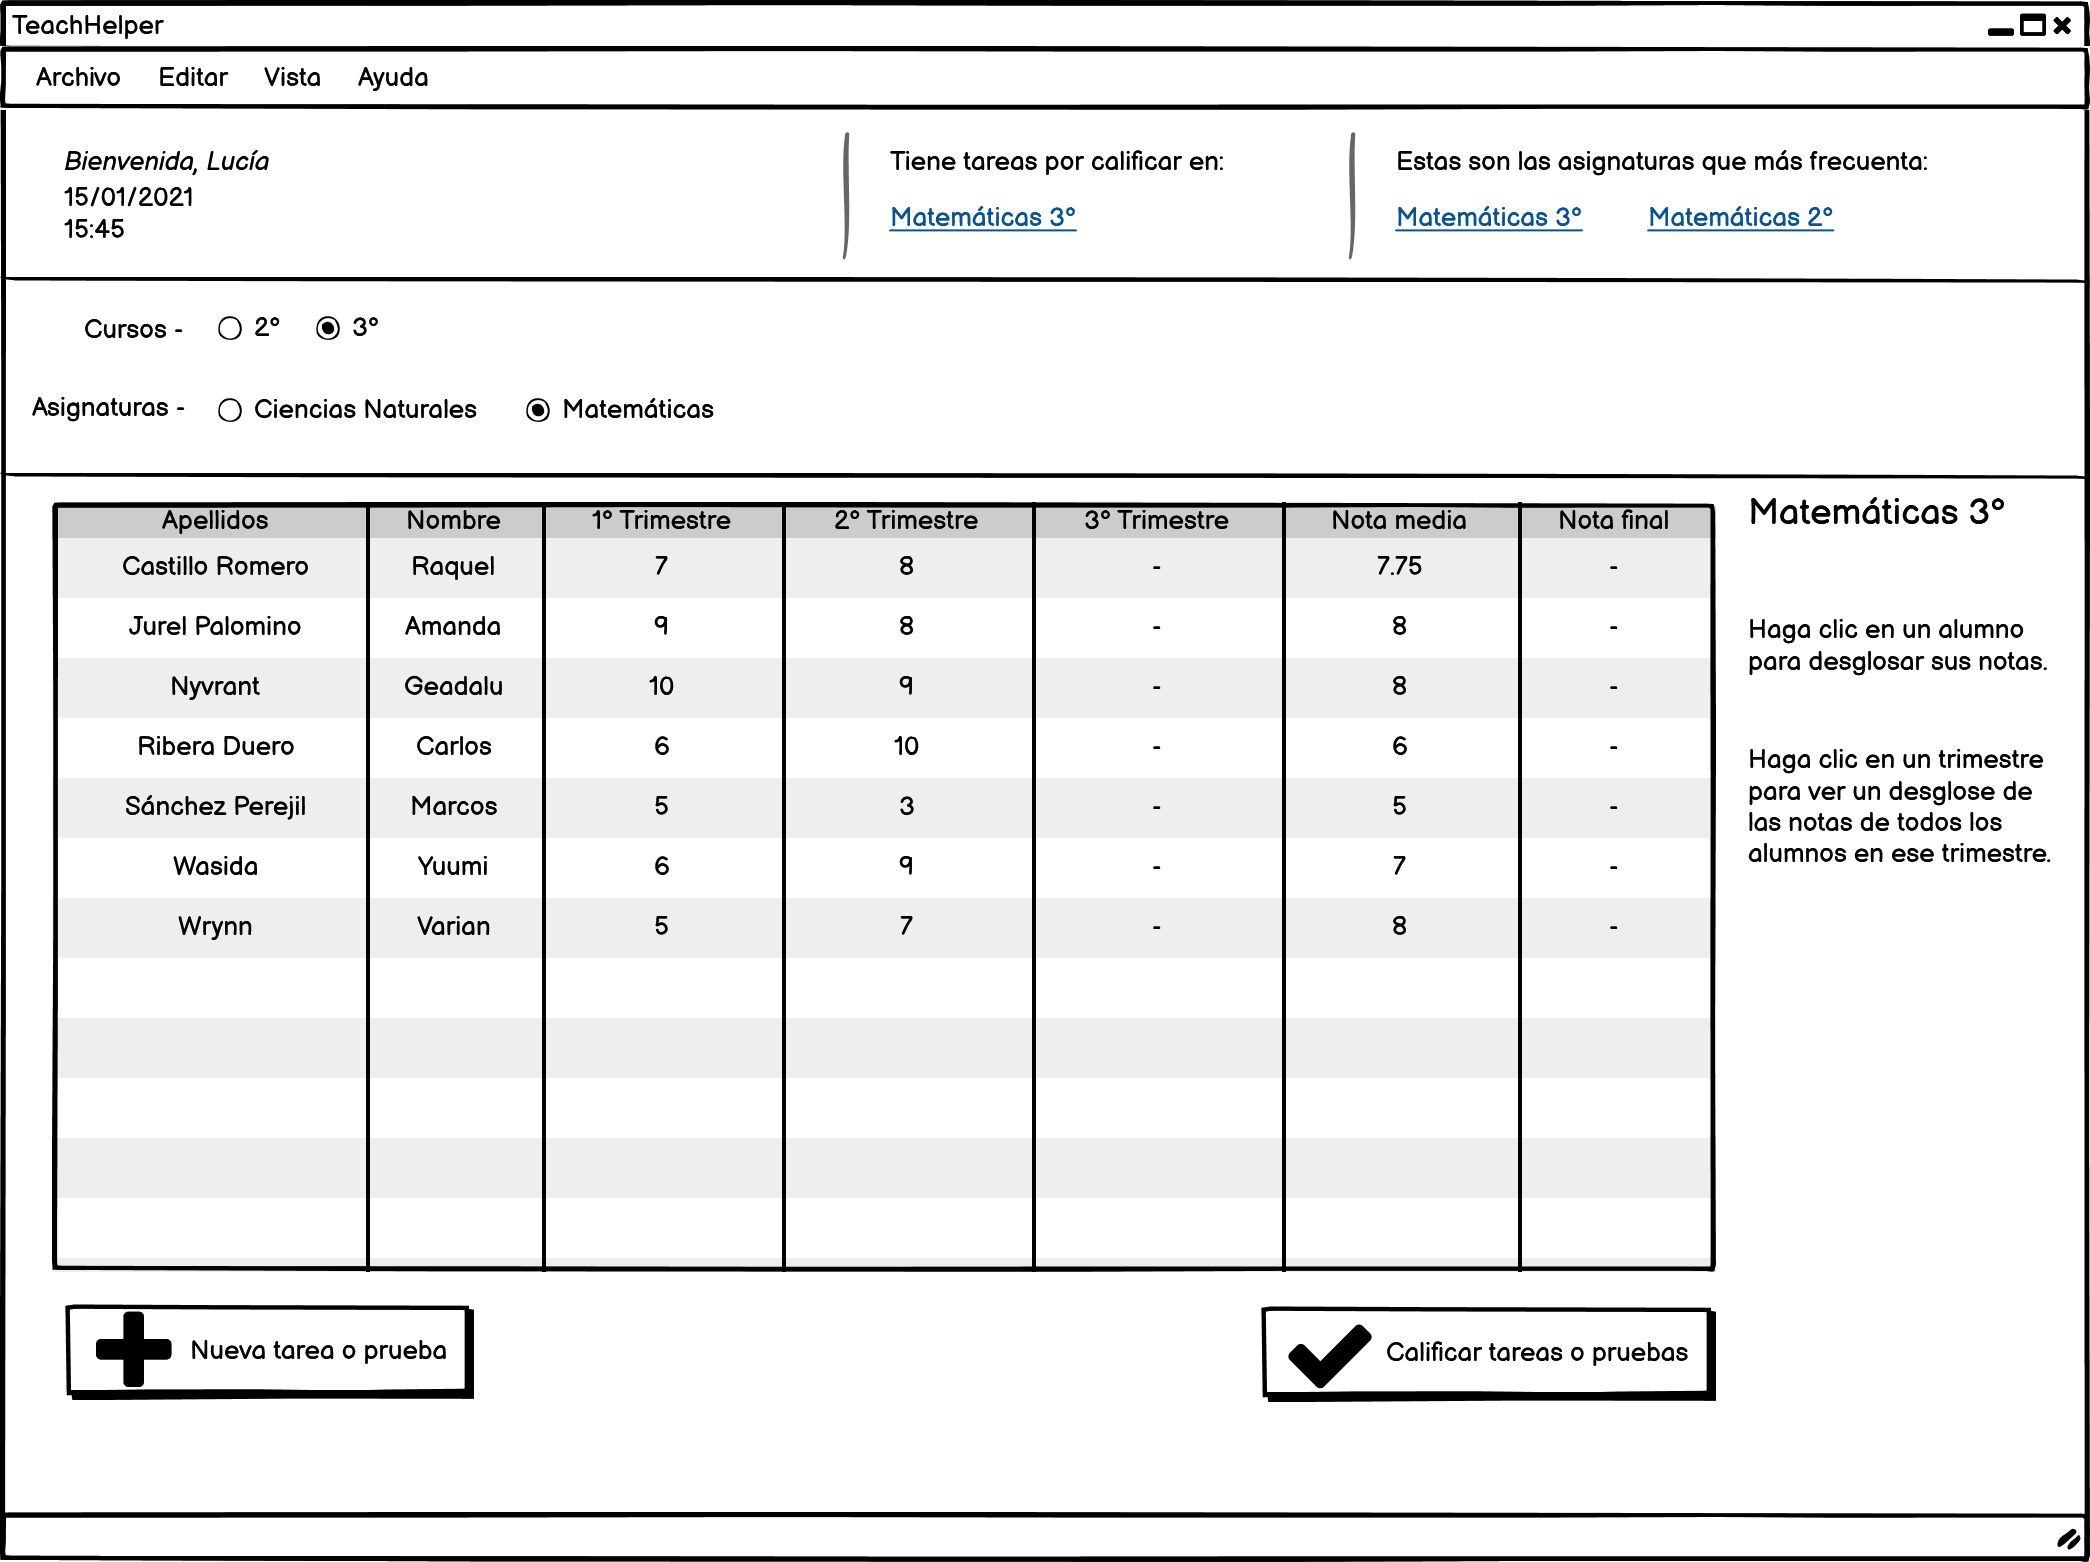
\includegraphics[width=1\linewidth]{figs/mockup_mainwindow.png}
\caption{Prototipo de la ventana principal.}
\label{Fig:mockup_mainwindow}
\end{figure}

\begin{figure}[h]
\centering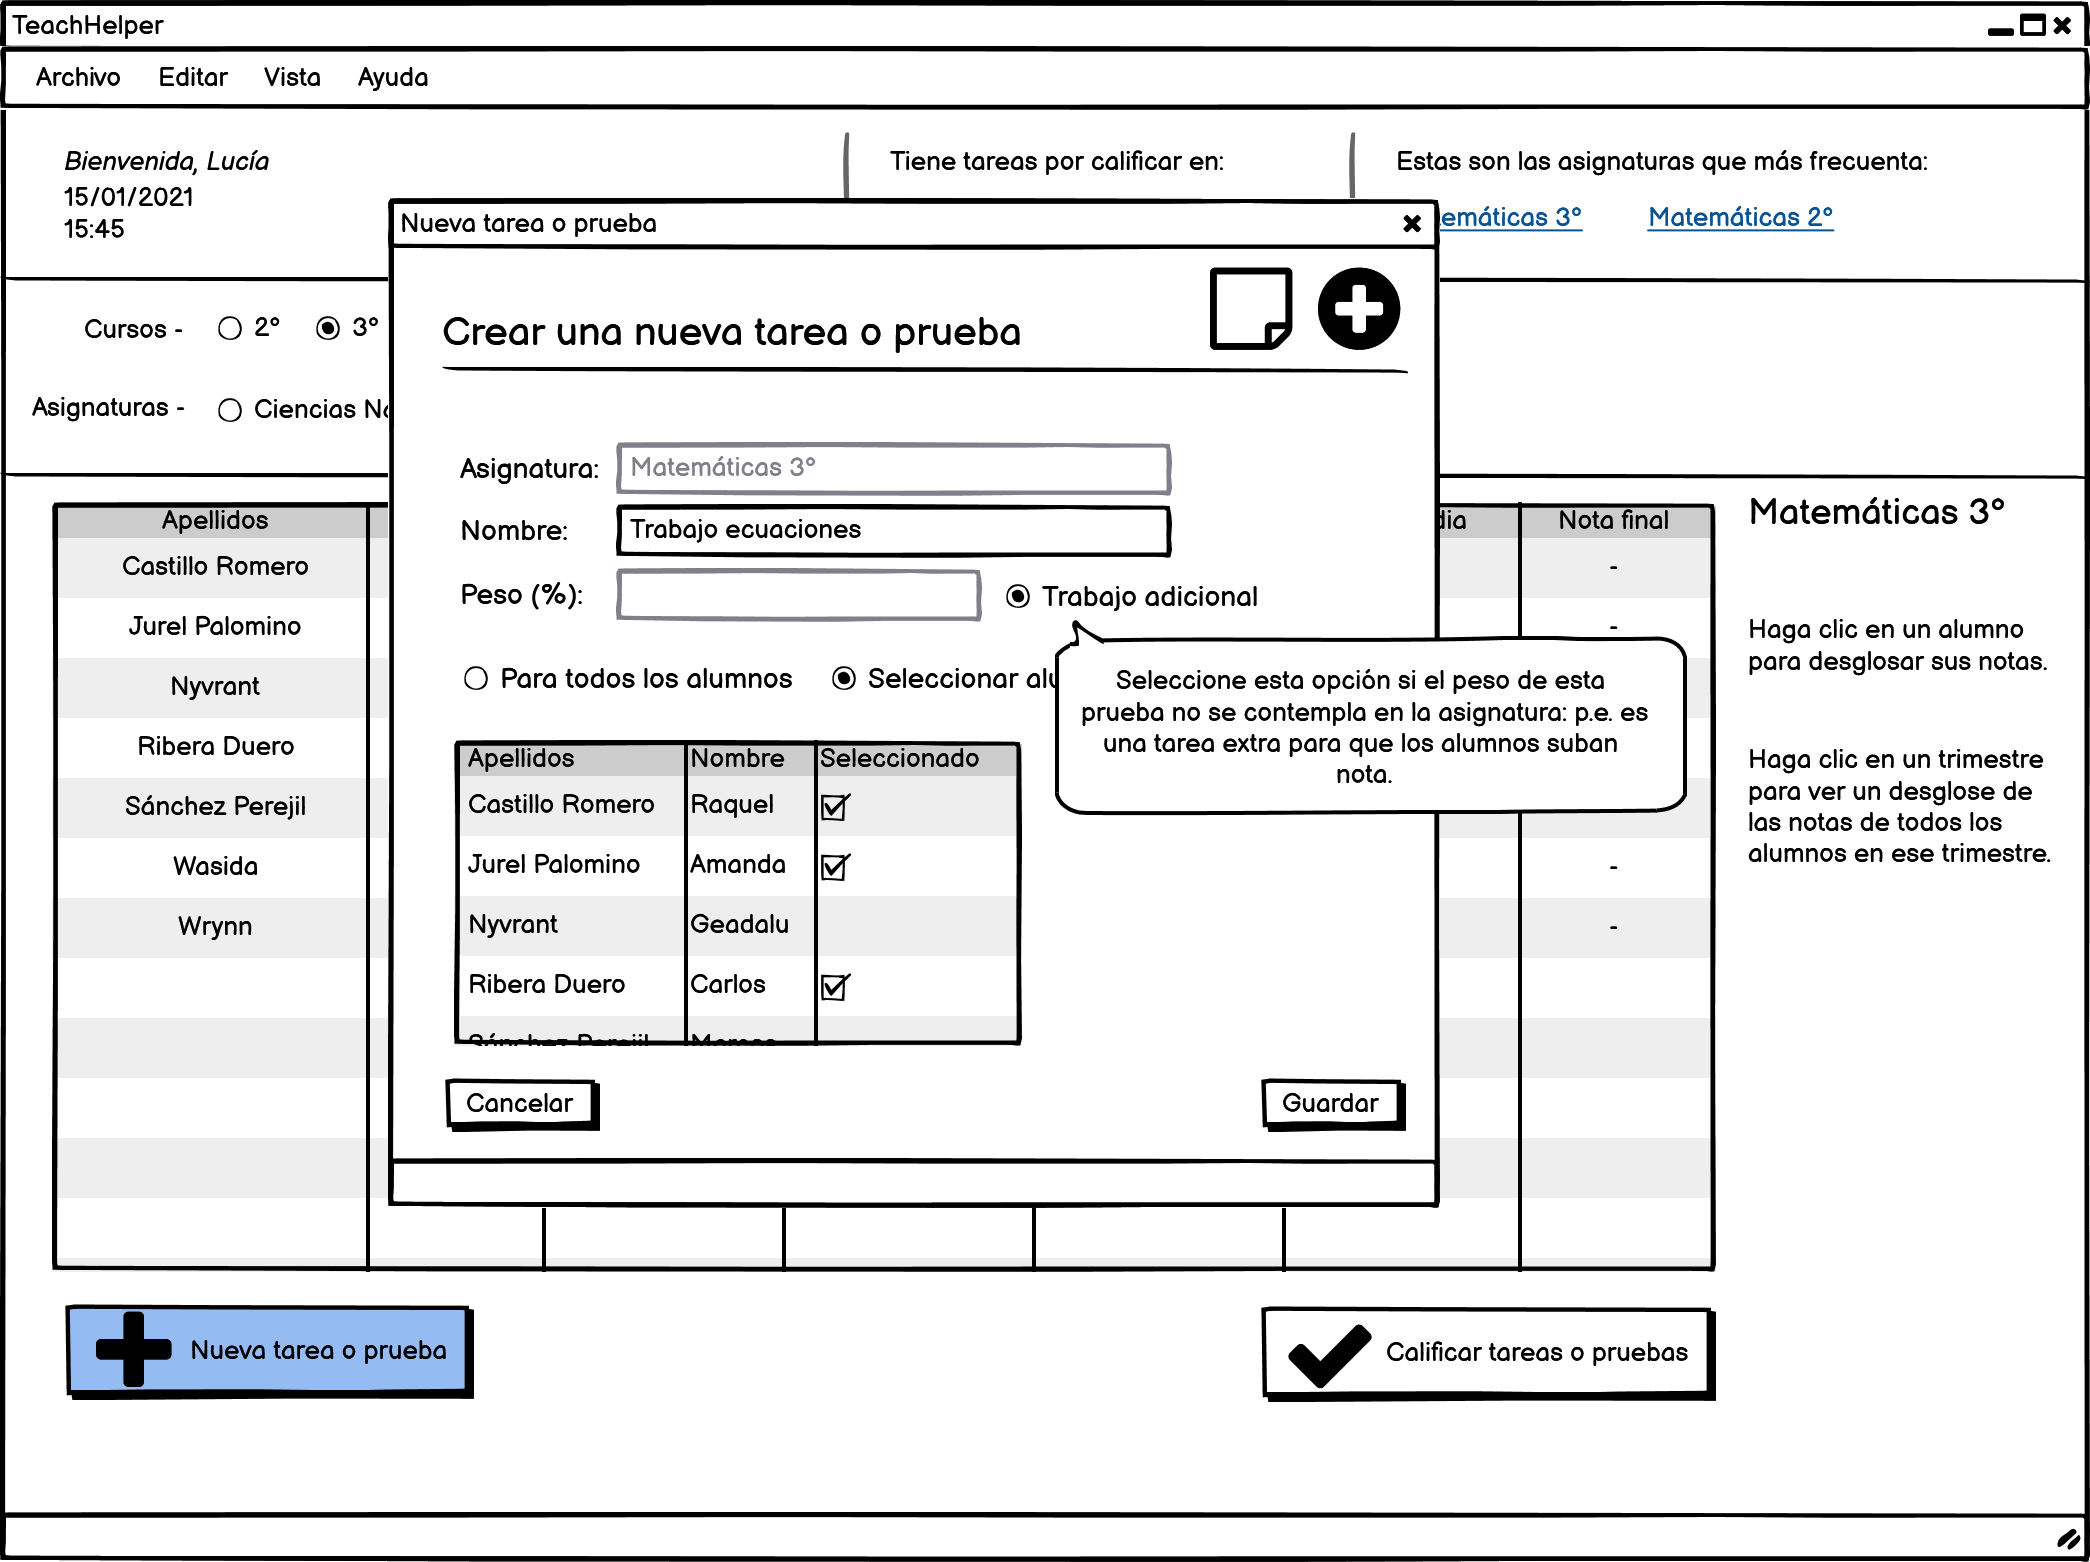
\includegraphics[width=1\linewidth]{figs/mockup_nuevatarea.png}
\caption{Prototipo de la creación de nuevas tareas o pruebas.}
\label{Fig:mockup_nuevatarea}
\end{figure}

\begin{figure}[h]
\centering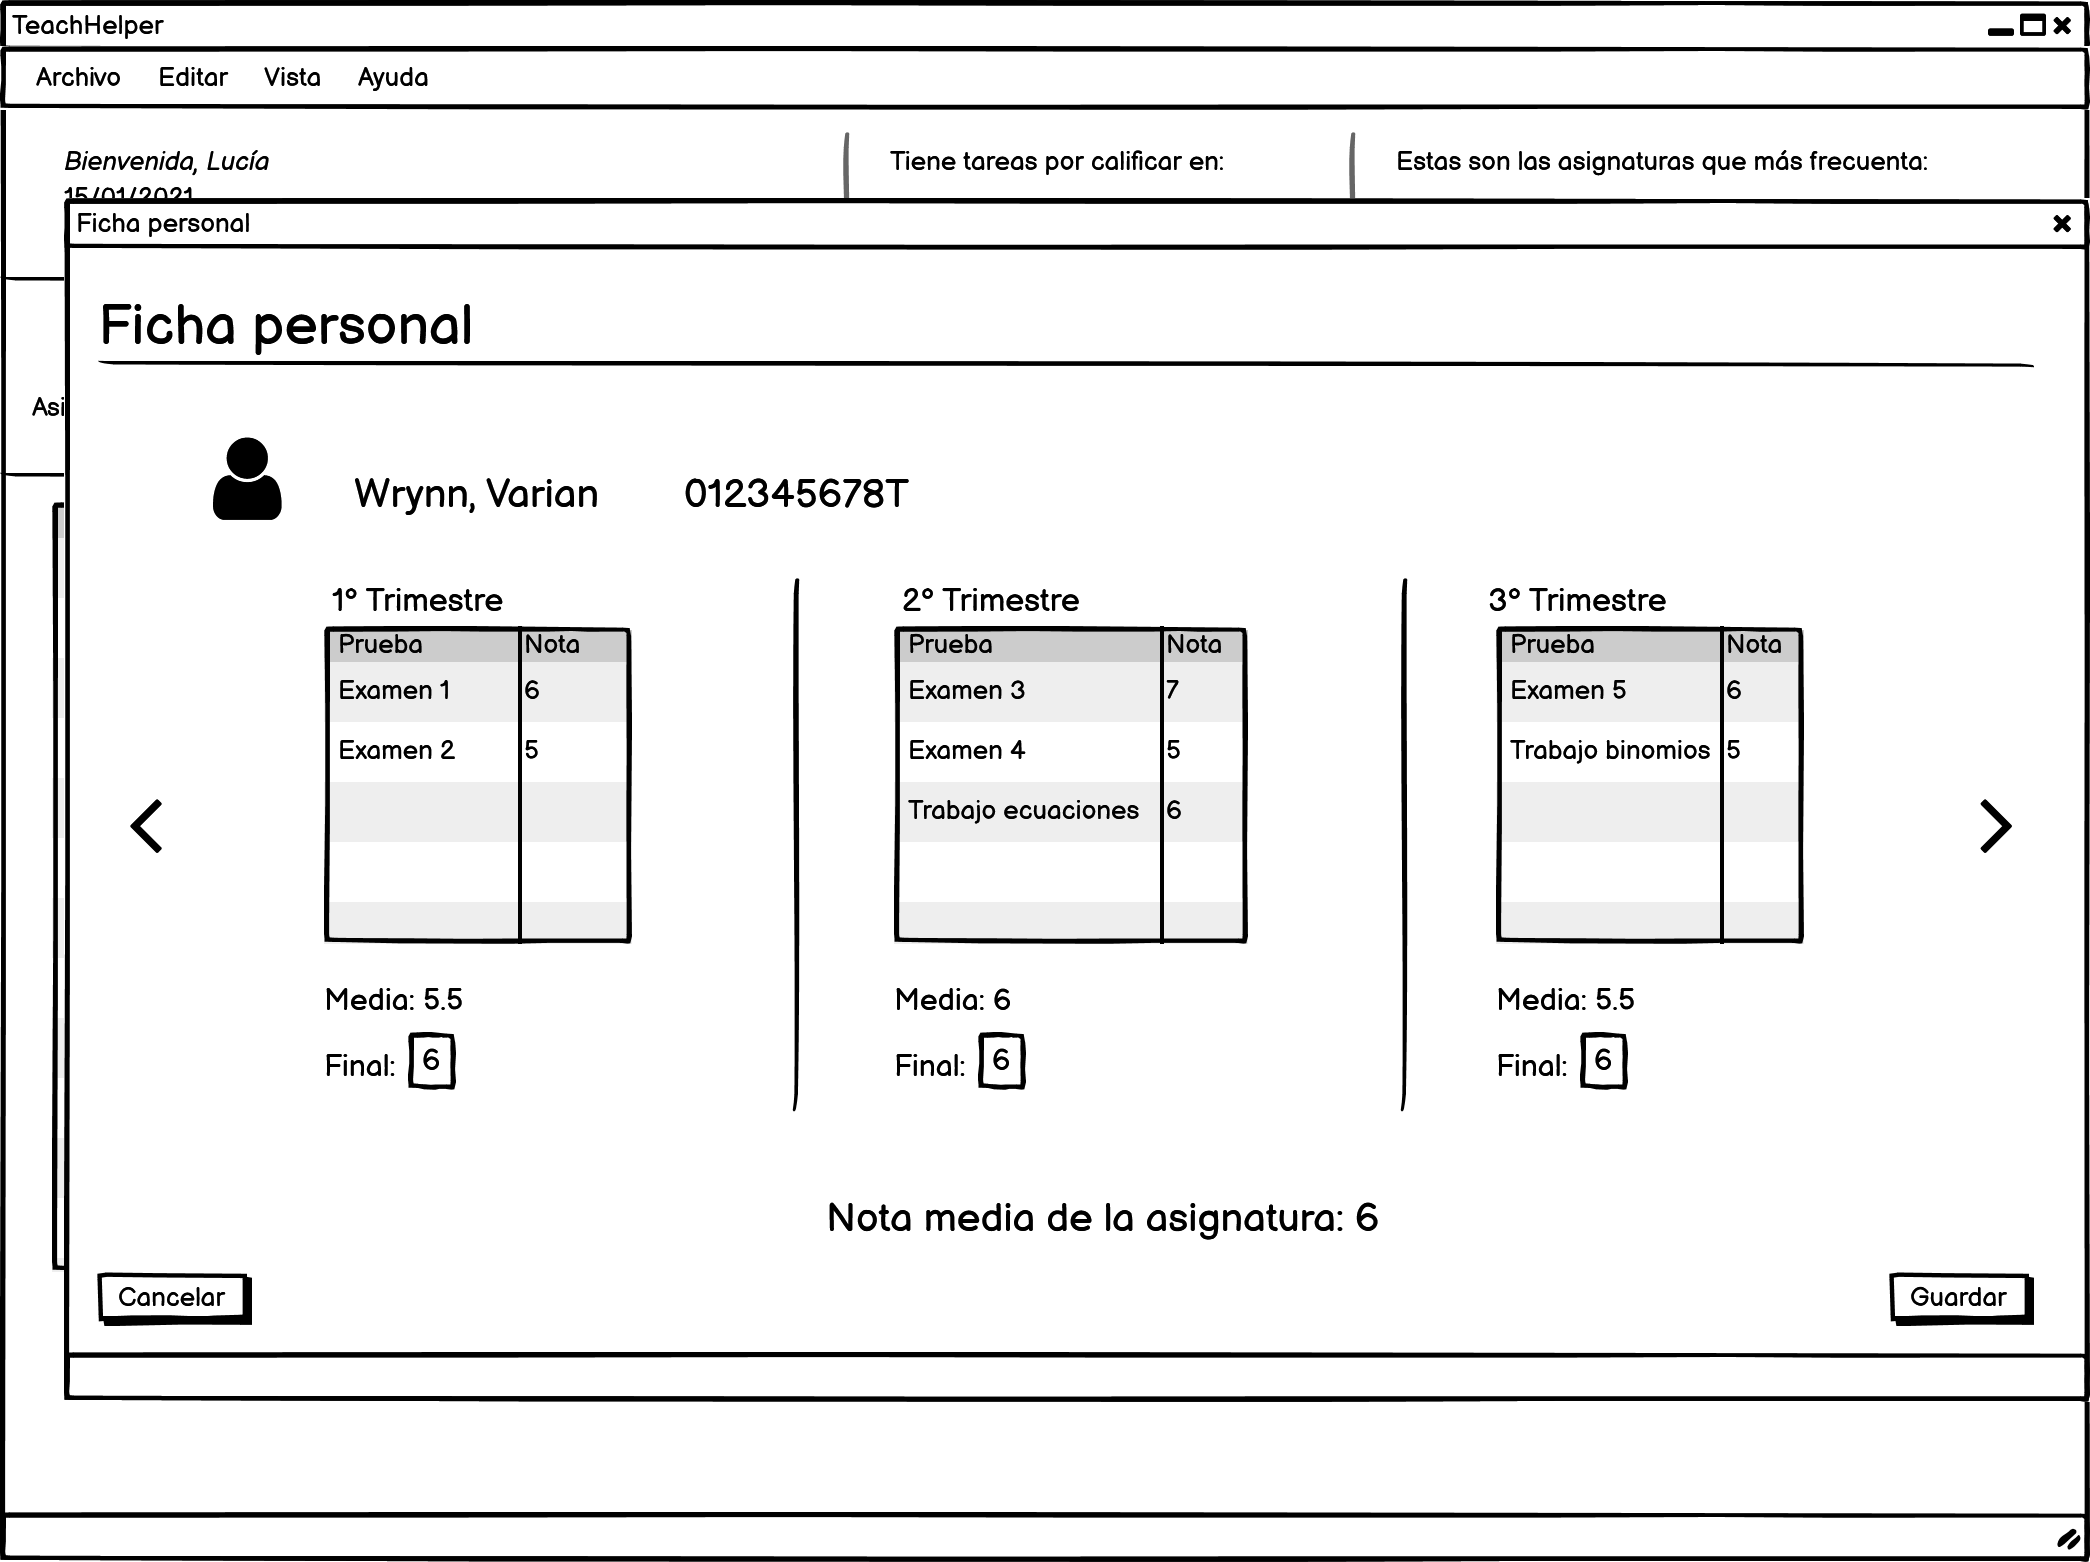
\includegraphics[width=1\linewidth]{figs/mockup_informealumno.png}
\caption{Prototipo del informe del alumnado.}
\label{Fig:mockup_informealumno}
\end{figure}


\section{Marco tecnológico de trabajo}

En esta sección se detallan las tecnologías usadas para el desarrollo de la aplicación.

\subsection{Java}
En la fase de Inicio del proyecto se estudió qué lenguaje de programación utilizar para su desarrollo. Al principio se propuso C\#, pero debido a las restricciones de horario de la desarrolladora y su previo conocimiento de Java (fuente: \cite{java}), se optó finalmente por el segundo.

Otra de las razones por las que se decantó por Java para realizar el proyecto fue la facilidad con la que se crean y modifican las interfaces gráficas con este lenguaje, concretamente si se usa un \gls{ide}.

A continuación se muestra una lista describiendo brevemente las librerías externas que se han usado en el desarrollo de este proyecto.
\begin{itemize}
	\item \textbf{Apache Poi}: permite crear y modificar archivos Microsoft Excel \cite{apachepoi}.
	\item \textbf{JFreeChart}: crea diagramas y gráficos y permite personalizarlos de varias maneras \cite{jfreechart}.
\end{itemize}

\subsection{Git y GitHub}
Se ha usado una herramienta de control de versiones llamada Git (fuente: \cite{git}). Esta herramienta permite subir el código a un repositorio, elegir los cambios que se quieren subir y deshacer los que se han hecho en caso de error. Ha sido de gran ayuda para gestionar el código y las iteraciones correctamente.

Este es el enlace al proyecto en GitHub: https://github.com/Geadalu/MisNotasCode.

Otra razón por la que se ha optado por Git es porque, desde su página web \url{www.github.com}, permite un control de "Issues" o problemas (ver figura \ref{Fig:issues_github}). Esto se ha usado de manera constante para tener mejor control de los errores que iban saliendo en el programa tras las iteraciones de desarrollo.

\begin{figure}[h]
\centering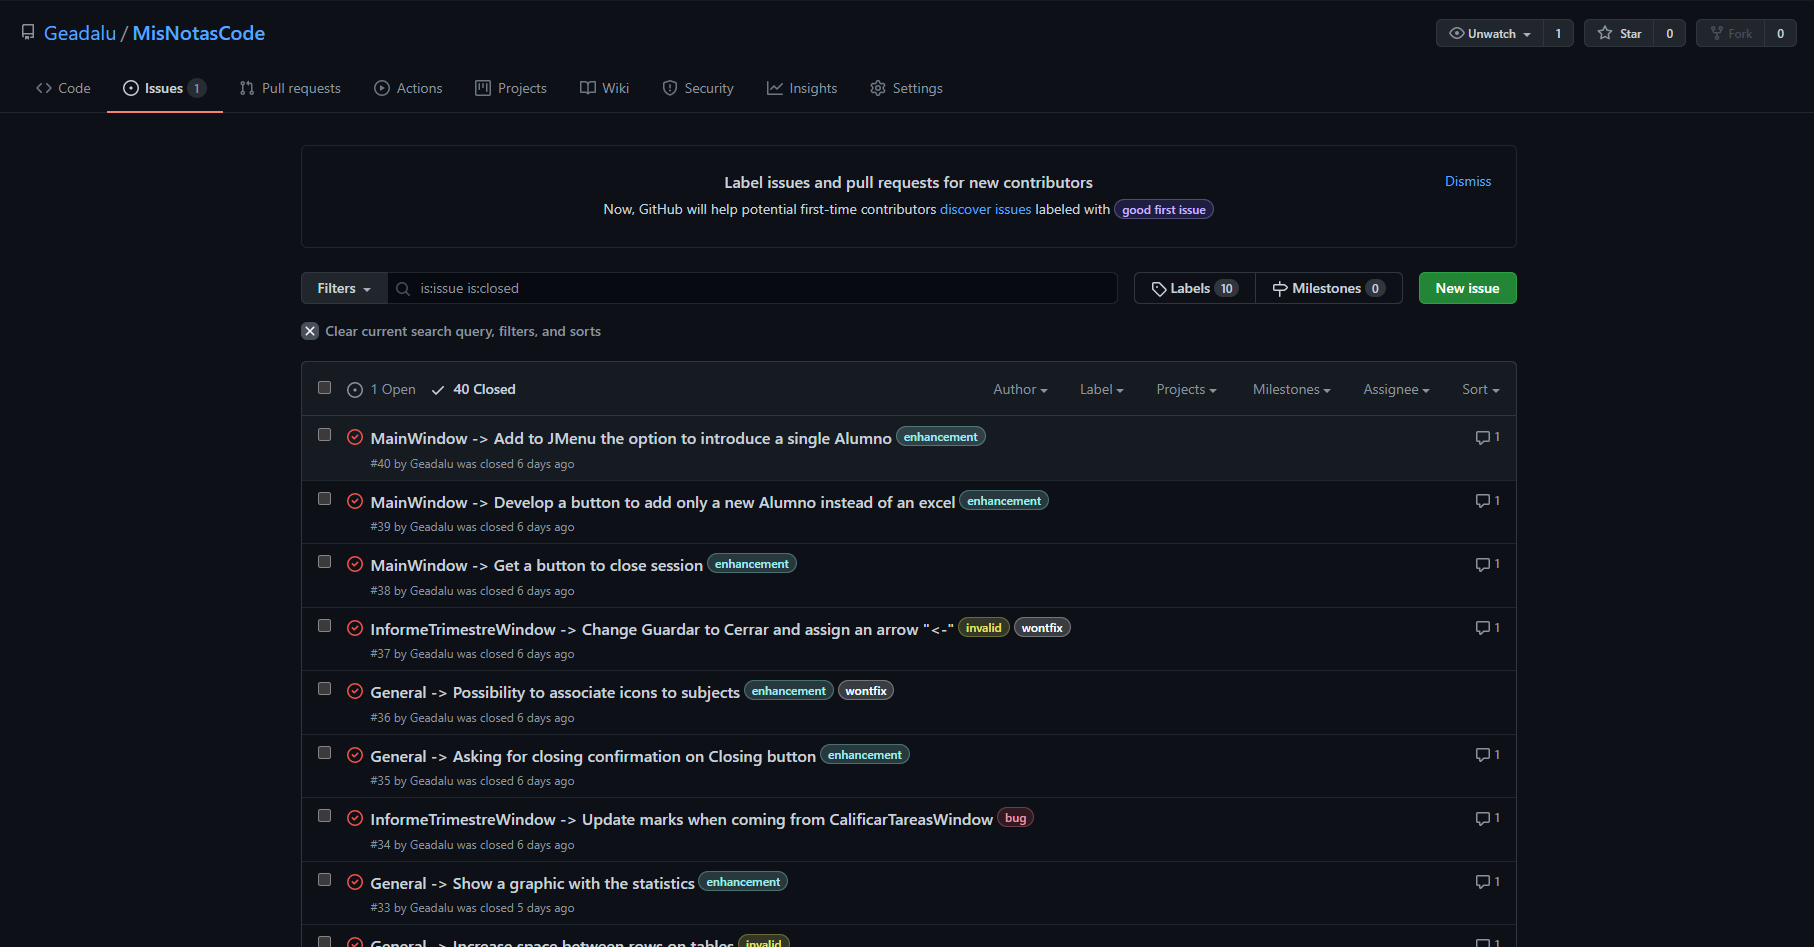
\includegraphics[width=1\linewidth]{figs/github.png}
\caption{Herramienta "Issues" de GitHub. Fuente: \cite{github}}
\label{Fig:issues_github}
\end{figure}

Por último, cabe destacar que también se ha usado la herramienta "Releases", que permite realizar lanzamientos de la aplicación, de manera que los usuarios que visiten el repositorio identificarán rápidamente cuál es la versión que pueden instalarse y ejecutar.


\subsection{Balsamiq Wireframes}
\label{sub:balsamiq}
Para realizar en la fase de Elaboración las maquetas de las interfaces (ver figura \ref{Fig:mockup_mainwindow}), se ha usado la aplicación Balsamiq Wireframes (fuente: \cite{balsamiq}. Esto permite modelar las interfaces de una manera fácil y sencilla. Permite hacer modelos de interfaces para ordenador, tablet y smartphone, y cuenta con una variedad de elementos que se pueden llamar entre sí para realizar una demo.

\subsection{Texmaker y Overleaf}
Se ha optado por los editores de textos Texmaker (ver figura \ref{Fig:texmaker}) y Overleaf para escribir este documento. Texmaker es una apliación de escritorio, que permite escribir y compilar en \LaTeX{}, que es el sistema de composición de textos mediante el cual se ha creado esta memoria.

Texmaker cuenta con el paquete LatexMk, que automatiza la compilación de todas las partes del documento: texto, bibliografía y referencias, y genera el resultado final en un PDF.

Overleaf (fuente: \cite{overleaf}) es, a su vez, un editor de texto para \LaTeX{}, pero web. Se ha decidido usar este cuando se ha tenido que cambiar de sitio de trabajo.

\begin{figure}[h]
\centering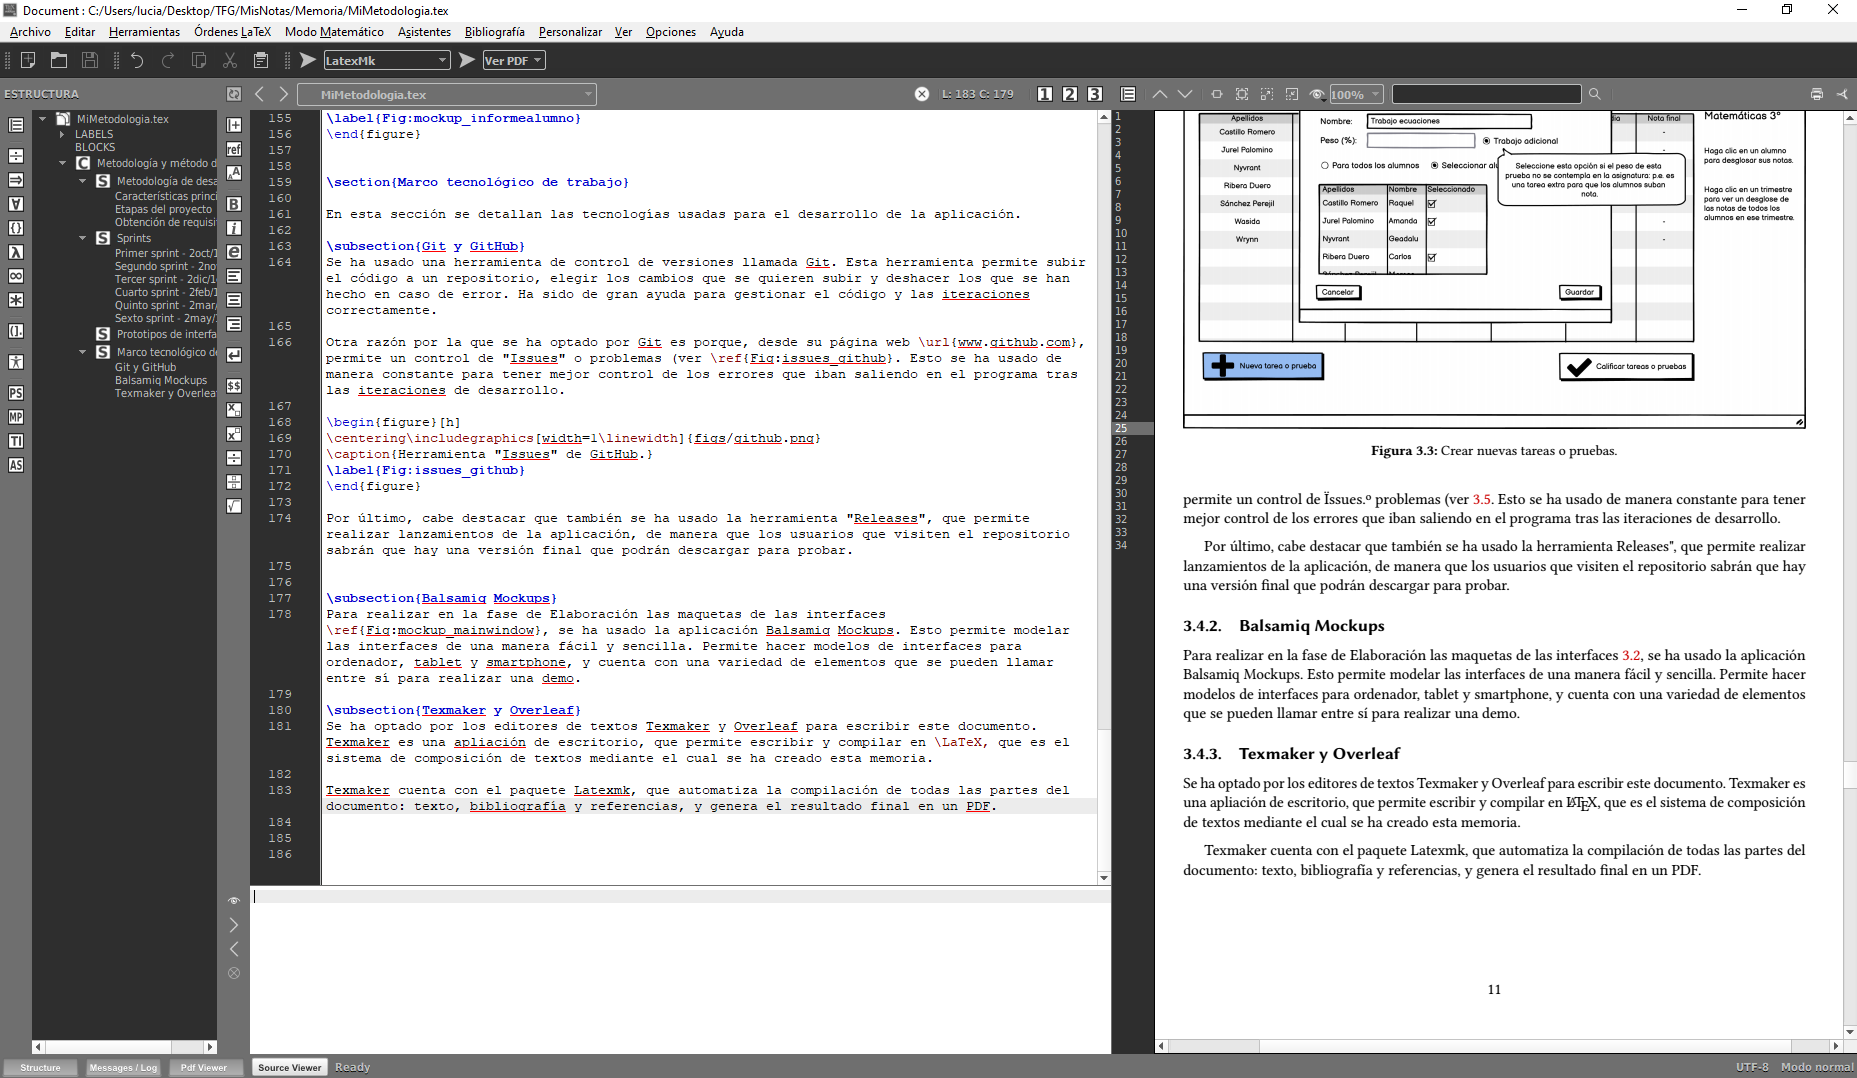
\includegraphics[width=1\linewidth]{figs/Texmaker.png}
\caption{Interfaz del editor de texto Texmaker. Fuente: \cite{texmaker}}
\label{Fig:texmaker}
\end{figure}


\subsection{NetBeans IDE}
Para la escritura de todo el código se ha usado el \gls{ide} gratuito NetBeans (ver figura \ref{Fig:netbeans}).
Este \gls{ide} cuenta con una potente herramienta para realizar las interfaces de los programas en Java, además, es altamente personalizable y tiene conexión con Git al repositorio de GitHub, de tal manera que, en un vistazo, se pueden ver las clases que han cambiado respecto a la versión que hay en GitHub.

\begin{figure}[h]
\centering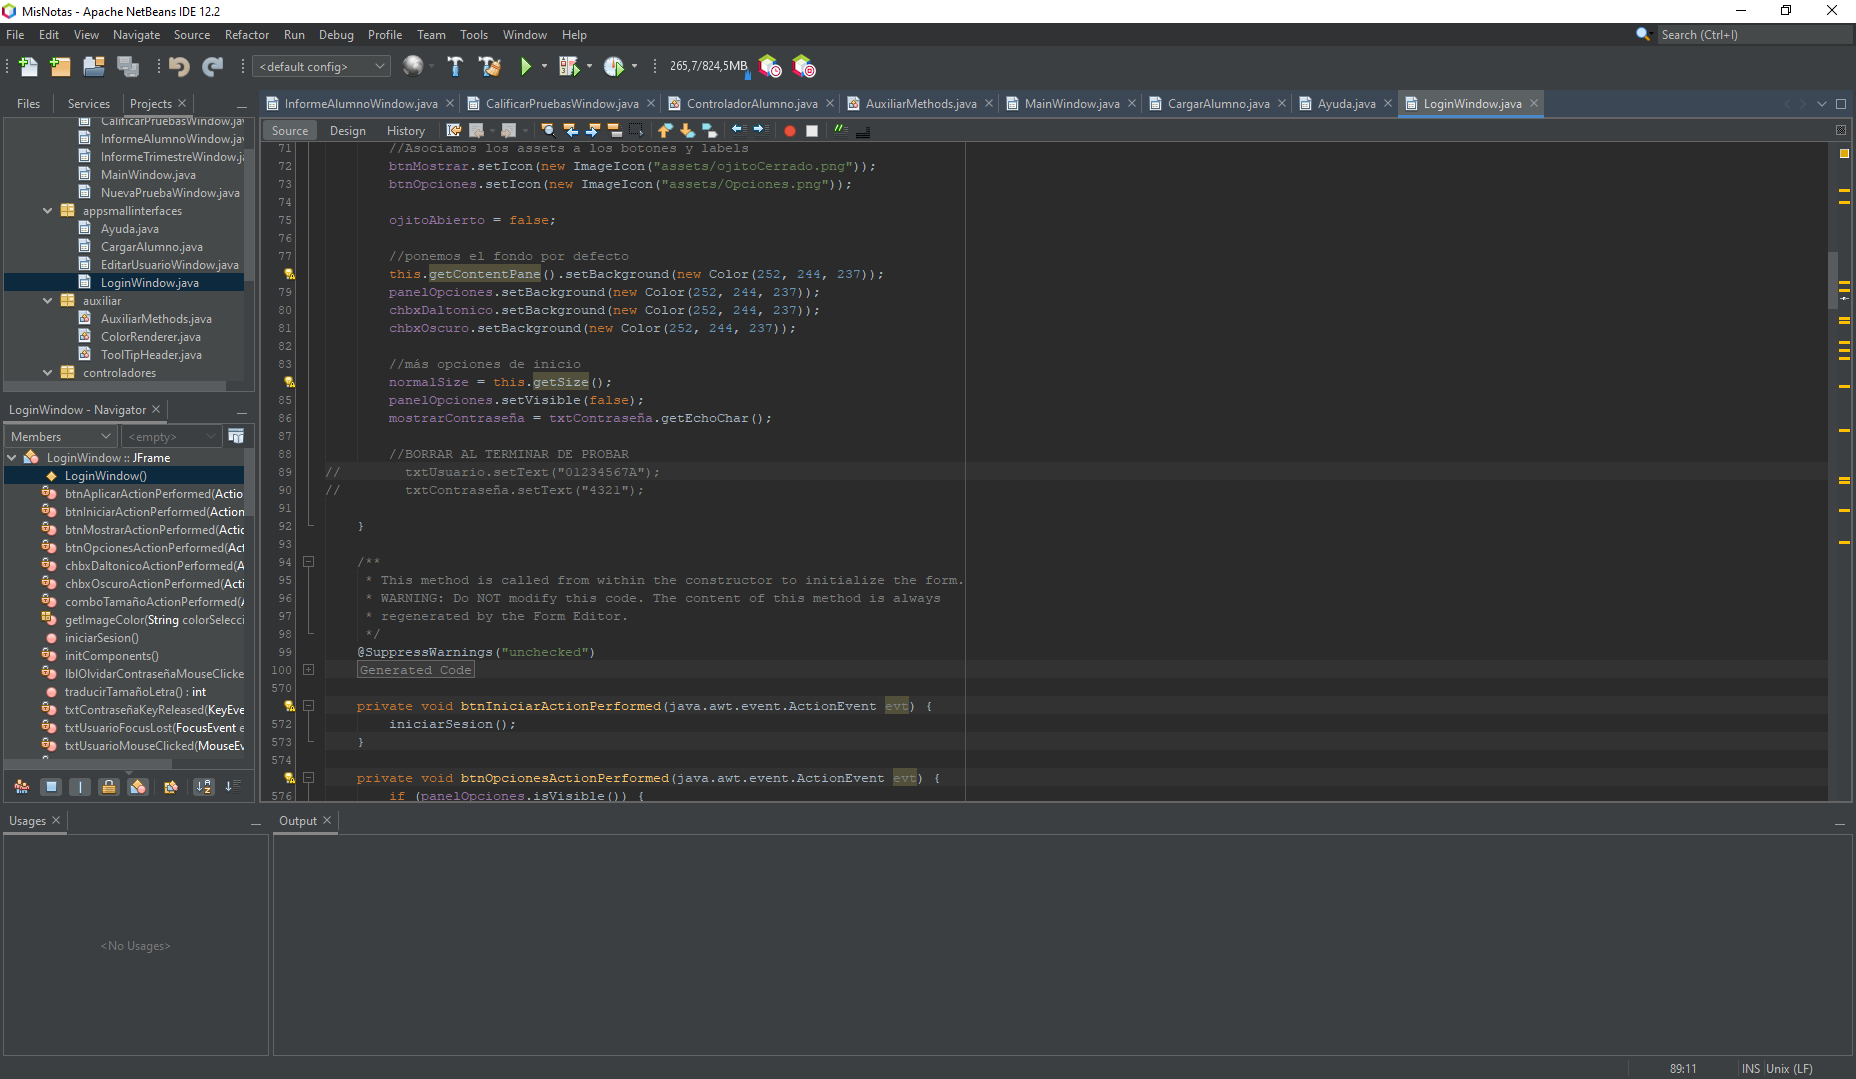
\includegraphics[width=1\linewidth]{figs/netbeans.png}
\caption{Interfaz de NetBeans IDE. Fuente: \cite{netbeans}}
\label{Fig:netbeans}
\end{figure}


\subsection{Procreate}
\label{sub:procreate}
Para el diseño de los iconos e imágenes que se han creado, se ha usado la aplicación de dibujo profesional Procreate (ver figura \ref{Fig:procreate}).

Es una aplicación sencilla e intuitiva que cuenta con varias herramientas para composición de dibujo y pintura.

\begin{figure}[h]
\centering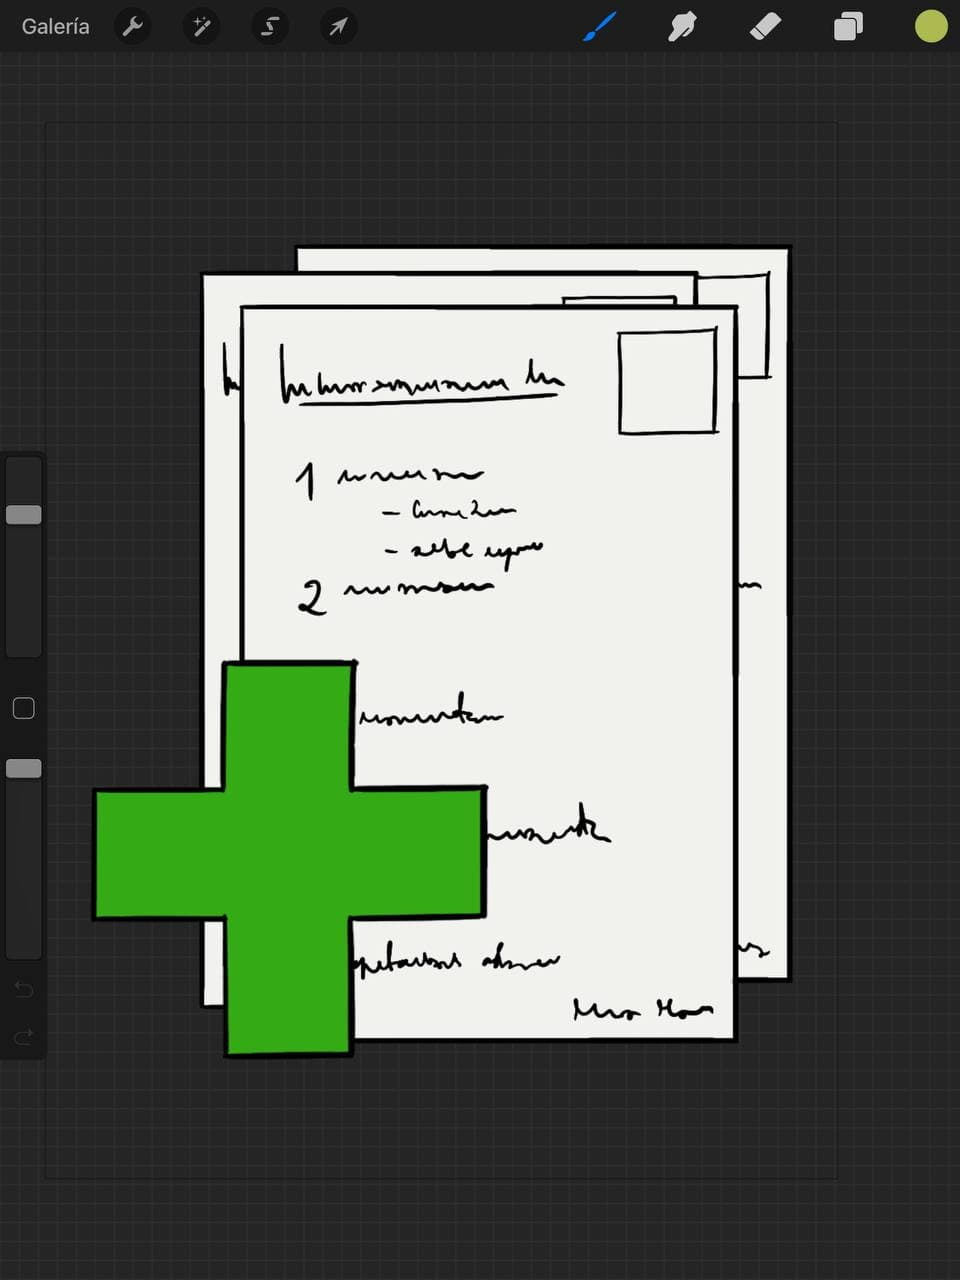
\includegraphics[width=0.5\linewidth]{figs/procreate.jpg}
\caption{Interfaz de dibujo de Procreate. Fuente: \cite{procreate}}
\label{Fig:procreate}
\end{figure}


\subsection{MySQL Workbench}
\label{sub:mysql}
Para la creación y gestión de la base de datos, se ha optado por MySQL Workbench (ver figura \ref{Fig:mysql}). Esta herramienta ha sido verdaderamente útil a la hora de gestionar todos los cambios que se han tenido que ir haciendo a medida que el proyecto iba creciendo, debido a la facilidad de uso y las funcionalidades que posee.

\begin{figure}[h]
\centering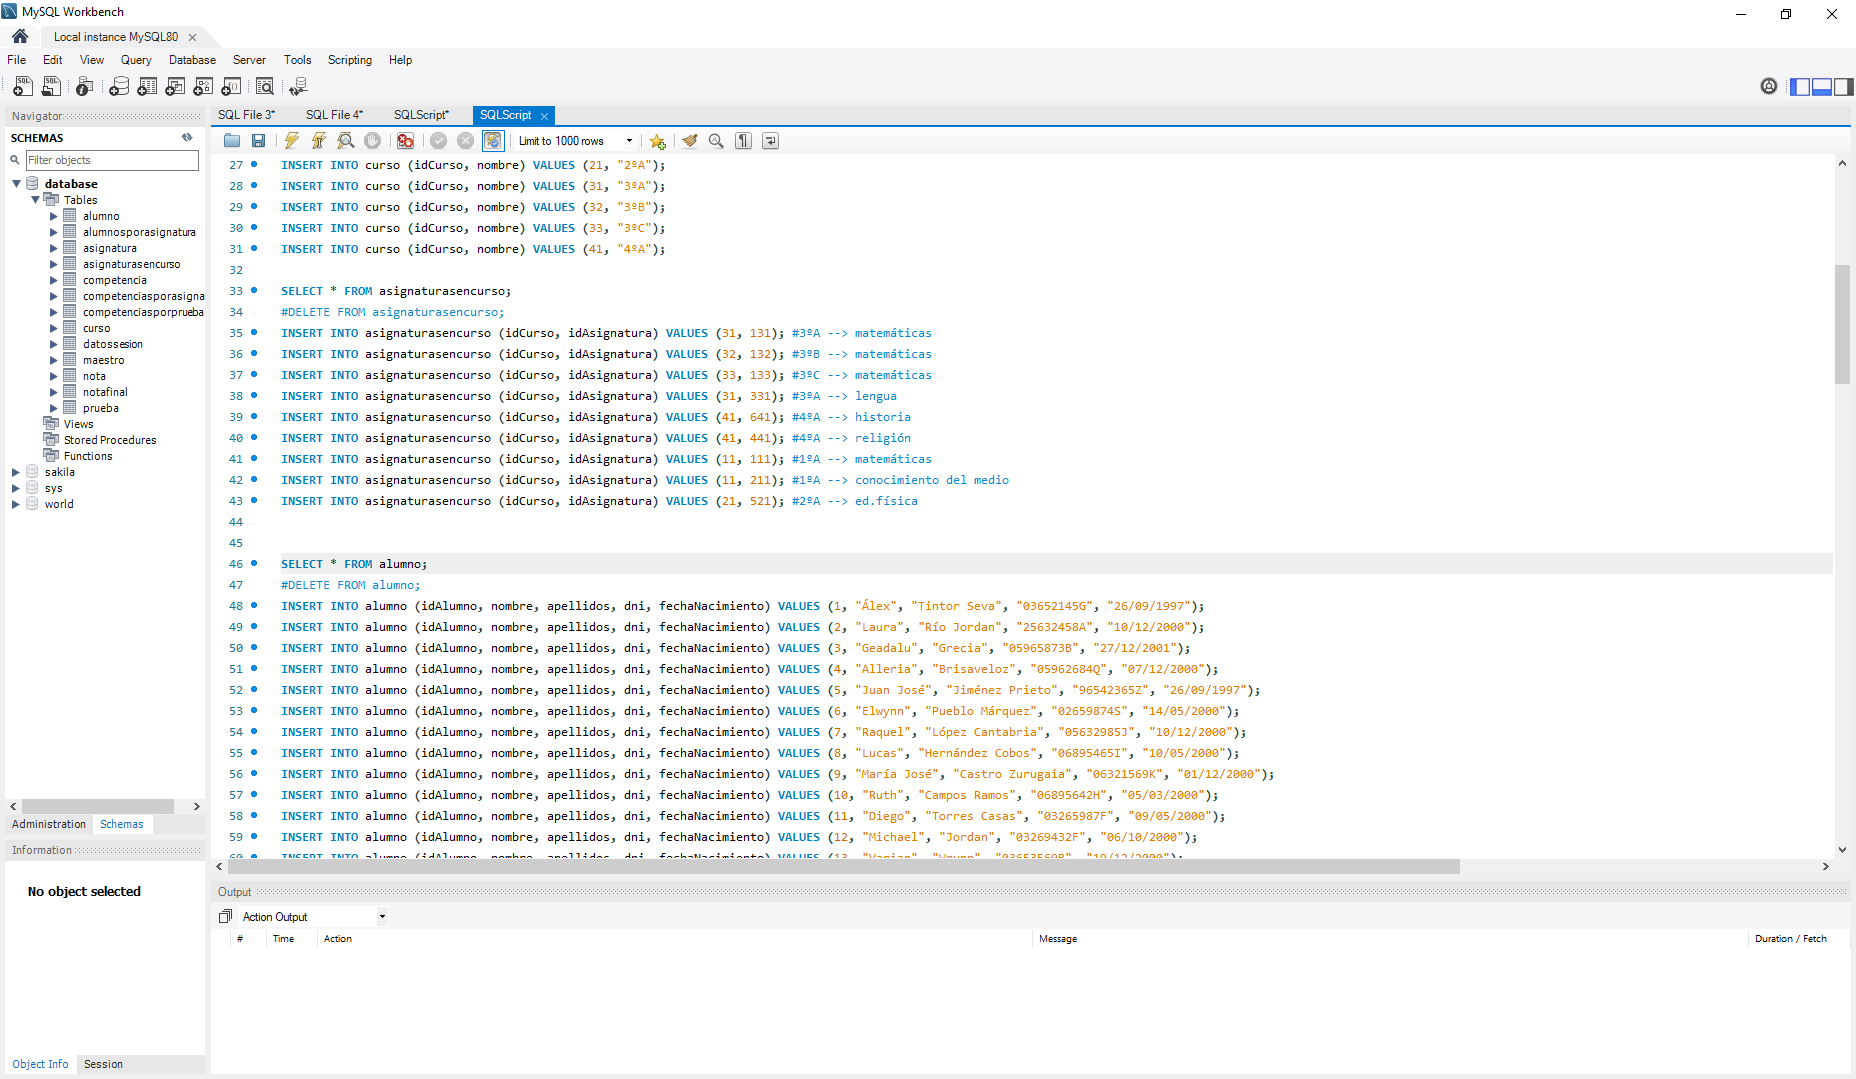
\includegraphics[width=1\linewidth]{figs/mysql.png}
\caption{Interfaz de MySQL Workbench. Fuente: \cite{mysql}}
\label{Fig:mysql}
\end{figure}


\subsection{Otras herramientas}
Cabe mencionar brevemente el uso de otras herramientas que han sido útiles en el desarrollo de este proyecto:
\begin{itemize}
	\item \textbf{tablesgenerator.com:} Como ayuda para la generación de tablas en este documento, se ha usado la herramienta web \url{https://www.tablesgenerator.com/}. Esta página permite crear una tabla de manera visual y generar el código \LaTeX{} correspondiente.
	\item \textbf{paint.net:} es un programa de escritorio para la edición de imágenes de manera básica. Se ha usado para cambiar el tamaño de las imágenes creadas con Procreate o de las sacadas de internet.
	\item \textbf{app.diagrams.net:} potente herramienta web usada para crear todos los diagramas de este documento.
\end{itemize}


\section{Análisis de costes}
\label{sec:analisiscostes}
Como parte de la fase de Inicio de este proyecto, se ha realizado un análisis de costes teniendo en cuenta las tecnologías que se fueran a usar, el tiempo estimado para la finalización del proyecto y otros gastos.

En la mayor parte del desarrollo del proyecto se ha usado software gratuito. Este software incluye: Java, MySQL Workbench, tablesgenerator.com, paint.net, Texmaker y Overleaf, NetBeans IDE, Balsamiq Mockups y Git y Github, mencionados en los apartados anteriores.

Para realizar este análisis de costes, se han tenido en cuenta todas las herramientas y materiales de trabajo, así como el lugar en el que se ha desarrollado y el coste del personal.

En la figura \ref{tab:tablacostes} se muestra una tabla con el software que no ha sido gratuito, así como los diversos costes estimados para el proyecto.

\begin{table}[h]
\caption{Tabla del análisis de costes}
\label{tab:tablacostes}
\begin{tabular}{|l|c|c|c|c|}
\hline
\textbf{Recurso}                                                                                               & \multicolumn{1}{l|}{\textbf{Descripción}}                                                                                                                                         & \multicolumn{1}{l|}{\textbf{\begin{tabular}[c]{@{}l@{}}Precio por \\ unidad\end{tabular}}} & \multicolumn{1}{l|}{\textbf{Unidades}} & \multicolumn{1}{l|}{\textbf{Total}} \\ \hline
\textbf{\begin{tabular}[c]{@{}l@{}}MSI GTX 1060 GAMING X \\ 6GB GDDR5\end{tabular}}                            & \begin{tabular}[c]{@{}c@{}}Tarjeta gráfica instalada\\ en el terminal de trabajo\end{tabular}                                                                                     & 274,98€                                                                                    & 1                                      & 274,98€                             \\ \hline
\textbf{\begin{tabular}[c]{@{}l@{}}Toshiba P300 3.5" 1TB \\ 7200RPM SATA 3\end{tabular}}                       & \begin{tabular}[c]{@{}c@{}}Disco duro instalado\\ en el terminal de trabajo\end{tabular}                                                                                          & 43,99€                                                                                     & 1                                      & 43,99€                              \\ \hline
\textbf{\begin{tabular}[c]{@{}l@{}}Kingston HyperX Fury Black \\ DDR4 2400 PC4-19200 \\ 8GB CL15\end{tabular}} & \begin{tabular}[c]{@{}c@{}}Memoria RAM instalada\\ en el terminal de trabajo\end{tabular}                                                                                         & 70,00€                                                                                     & 2                                      & 140,00€                             \\ \hline
\textbf{Intel Core i5-8400 2.8GHz BOX}                                                                         & \begin{tabular}[c]{@{}c@{}}Procesador instalado\\ en el terminal de trabajo\end{tabular}                                                                                          & 259,90€                                                                                    & 1                                      & 259,90€                             \\ \hline
\textbf{Otros componentes}                                                                                     & \begin{tabular}[c]{@{}c@{}}Otros componentes (cableado, \\ placa base, conector Internet, \\ fuente de alimentación, etc) \\ instalados en el terminal \\ de trabajo\end{tabular} & 230,64€                                                                                    & 1                                      & 230,64€                             \\ \hline
\textbf{Procreate}                                                                                             & \begin{tabular}[c]{@{}c@{}}Aplicación usada en el\\ desarrollo de las figuras\\ de la aplicación\end{tabular}                                                                     & 10,99€                                                                                     & 1                                      & 10,99€                              \\ \hline
\textbf{Alquiler de oficina}                                                                                   & \begin{tabular}[c]{@{}c@{}}Precio mensual del alquiler\\ de una oficina en Madrid\\ para realizar el trabajo\end{tabular}                                                         & 1000,00€                                                                                   & 6                                      & 6.000€                              \\ \hline
\textbf{Coste de personal}                                                                                     & \begin{tabular}[c]{@{}c@{}}Coste horario de la\\ desarrolladora del proyecto\end{tabular}                                                                                         & 9.98€                                                                                      & 350                                    & 3.493€                              \\ \hline
\textbf{Otros costes}                                                                                          & \begin{tabular}[c]{@{}c@{}}Se incluyen: tarifa de luz,\\ material de oficina, etc.\end{tabular}                                                                                   & 150.00€                                                                                    & 1                                      & 150.00€                             \\ \hline
\textbf{COSTE TOTAL}                                                                                           & Suma de la columna Total                                                                                                                                                          & \multicolumn{1}{l|}{}                                                                      & \multicolumn{1}{l|}{}                  & 10.603,50€                          \\ \hline
\end{tabular}
\end{table}


El coste total del proyecto se estima en 10.603,50€(Euros)
\chapter{Resultados}
\label{cap:Resultados}

En esta sección se describirá la aplicación del método de trabajo presentado en el capítulo \ref{cap:MiMetodologia} en este caso concreto, mostrando los elementos (modelos, diagramas, especificaciones, etc.) más importantes. Este apartado debe explicar cómo la metodología satisface los objetivos y requisitos planteados.

\chapter{Conclusiones}
\label{cap:conclusiones}
En este último capítulo se habla de las conclusiones extraídas de este trabajo y se proponen algunas vías para continuarlo o mejorarlo.

\section{Conclusiones}
En este trabajo se ha desarrollado una herramienta intuitiva y usable para una cómoda calificación de los docentes a su alumnado. Se han conseguido todos los objetivos propuestos en el capítulo \ref{cap:objetivo} e incluso se han añadido algunas funcionalidades nuevas que no se pensaron al principio.

En comparación a las aplicaciones existentes de las que se habló en el capítulo \ref{aplicacionesexistentes}, se considera que el resultado de este proyecto las ha mejorado en los siguientes puntos:
\begin{enumerate}
	\item \textbf{Privacidad de los datos}. Todas las aplicaciones que se investigaron tenían acceso a Internet. Si bien esto, para sus especificaciones, era necesario (debido a que todas ellas implementaban la capacidad de comunicación entre docente y alumnado), también supone un mínimo riesgo de filtración de datos. La aplicación desarrollada, al ser de escritorio, no encuentra ese problema y sus datos están completamente seguros.
	\item \textbf{Alta personalización de la interfaz gráfica}. A la hora de trabajar con un ordenador, hay algunas personas que necesitan aumentar el tamaño de la letra, o crear un mayor contraste entre los elementos que se muestran en la pantalla. Esta aplicación lo permite, posibilitando una sesión de trabajo lo más cómoda y agradable posible.
	\item \textbf{Control de competencias}. Si bien Additio \ref{sec:additio} era la única aplicación que permitía un control de competencias, en la aplicación desarrollada se permiten visualizar con mayor claridad en cualquier momento mediante la funcionalidad "Informe del trimestre".
\end{enumerate}

Para terminar, comentar que gracias a la prueba de usabilidad realizada, se puede concluir que el desarrollo ha sido un éxito, aunque podría mejorar en varios aspectos que se discuten en la sección a continuación.
	

\section{Propuestas de trabajo futuro}
\label{sec:trabajofuturo}
Como posible continuación del desarrollo de esta aplicación, se proponen a continuación varios puntos que añaden funcionalidades nuevas o mejoran las existentes.

Estas son ideas que han ido surgiendo a lo largo del desarrollo, y que podrían beneficiar a la aplicación de distintas maneras.

\begin{itemize}
	\item \textbf{Mejora de la interfaz gráfica}. En general, el aspecto de la aplicación es primitivo y simple. Esto es un importante aspecto a tener en cuenta puesto que podría aumentar el número de docentes que desearan utilizar esta aplicación, además de mejorar la experiencia de usuario.
	\item \textbf{Adición del rol de administrador}. En el momento de finalización de este proyecto solo hay un tipo de usuario que puede acceder a la aplicación, y este es el maestro. Sin embargo, se ha considerado que el sistema podría beneficiarse de la existencia de un rol de administrador, que accediera a una pantalla especial para cargar nuevas asignaturas y nuevos cursos al docente, y para que inicializara las aplicaciones para los docentes nuevos en el centro o cada inicio de curso.
	\item \textbf{Más opciones de personalización}. Varios de los comentarios recogidos en la prueba de usabilidad [\ref{sub:pruebausabilidad}] se orientan a la personalización. Se podría implementar un sistema para calificar de manera diferente, en lugar de solo con un número para la nota y un comentario, de manera menos sistemática para tener en cuenta otros aspectos aparte de la nota.
	\item \textbf{Posibilidad de apuntar si se ha hecho la tarea}. También se podría implementar un sistema que permita al docente apuntar los días que el alumno ha hecho la tarea para casa e incluso calificarla. También, en la propia ventana de calificación de tareas, si el alumno ha terminado o no haciendo esa tarea.
\end{itemize}

% -------------------------

% -------------------------
%
% OPT.: ANEXOS: Comentar si no se desean incluir.
%
% -------------------------
\appendix

% Tras este punto los capítulos se numeran con letras.
% Aquí todos los apéndices necesarios
\chapter{El primer anexo}
\label{cap:AnexoA}

En los anexos se incluirá de modo opcional material suplementario que podrá consistir en breves manuales, listados de código fuente, esquemas, planos, etc. Se recomienda que no sean excesivamente voluminosos, aunque su extensión no estará sometida a regulación por afectar esta únicamente al texto principal. 

\paragraph{Bibliografía}
Esta sección, que si se prefiere puede titularse «Referencias», incluirá un listado por orden alfabético (primer apellido del primer autor) con todas las obras en que se ha basado para la realización del TFG en las que se especificará: autor/es, título, editorial y año de publicación. Solo se incluirán en esta sección las referencias bibliográficas que hayan sido citadas en el documento. Todas las fuentes consultadas no citadas en el documento deberían incluirse en una sección opcional denominada <<Material de consulta>>, aunque preferiblemente estas deberían incluirse como referencias en notas a pie de página a lo largo del documento.

Se usará método de citación numérico con el número de la referencia empleada entre corchetes. La cita podrá incluir el número de página concreto de la referencia que desea citarse. Debe tenerse en cuenta que el uso correcto de la citación implica que debe quedar claro para el lector cuál es el texto, material o idea citado. Las obras referenciadas sin mención explícita o implícita al material concreto citado deberían considerarse material de consulta y por tanto ser agrupados como «Material de consulta» distinguiéndolas claramente de aquellas otras en las que si se recurre a la citación.

Cuando se desee incluir referencias a páginas genéricas de la Web sin mención expresa a un artículo con título y autor definido, dichas referencias podrán hacerse como notas al pie de página o como un apartado dedicado a las «Direcciones de Internet».

Todo el material ajeno deberá ser citado convenientemente sin contravenir los términos de las licencias de uso y distribución de dicho material. Esto se extiende al uso de diagramas y fotografías. El incumplimiento de la legislación vigente en materia de protección de la propiedad intelectual es responsabilidad exclusiva del autor del trabajo independientemente de la cesión de derechos que este haya convenido. De este modo será responsable legal ante cualquier acción judicial derivada del incumplimiento de los preceptos aplicables. Así mismo ante dicha circunstancia los órganos académicos se reservan el derecho a imponer al autor la sanción administrativa que se estime pertinente. 

\paragraph{Índice temático}
Este índice es opcional y se empleará como índice para encontrar los temas tratados en el trabajo. Se organizará de modo alfabético indicando el número de página(s) en el que se aborda el tema concreto señalado.
 % Apéndice A (opcionales)

%---

%--- BACKMATTER
\backmatter
% -------------------------
%
% BIBLIOGRAFÍA
%
% -------------------------
% OJO: Todas  las referencias deben estar citadas en el texto)
% EDITAR: Comentar línea siguiente
\nocite{*} % INCLUIDO para ver cómo queda, pero comentar en versión final.

\phantomsection  % OJO: Ojo necesario con hyperref.
\addcontentsline{toc}{chapter}{\bibname} % Añade la bibliografía al Índice de contenidos.
%---
% Opción 1: Bibliografía con todas las fuentes en un apartado.
%---
\printbibliography
%---

%---
% Opción 2: Bibliografía con secciones separadas.
%---
%\printbibheading
%\printbibliography[heading=subbibliography,type=online,title={Fuentes online}]
%\printbibliography[heading=subbibliography,nottype=online,title={Fuentes no online}]
% -------------------------

% -------------------------
%
% OPT.: ÍNDICE TEMÁTICO: Comentar si no se desean incluir.
%
% -------------------------
% CONSEJO: Incluir los comandos mientras se escribe cada capítulo ya que hacerlo al final resulta tedioso.
\cleardoublepage
\phantomsection % OJO: Ojo necesario con hyperref.
\addcontentsline{toc}{chapter}{\indexname} % Añade al Índice de contenidos.

%---
% Impresión de Índice Temático (comentar para eliminar)
%---
\printindex  % Facilitado por makeidx (opcional, si no se usa no se imprime)
%---
\end{document}